\renewcommand{\thefigure}{\textsc{a}\arabic{figure}}
\renewcommand{\theequation}{\textsc{a}\arabic{equation}}
\renewcommand{\thetable}{\textsc{a}\arabic{table}}
\setcounter{figure}{0}
\setcounter{equation}{0}

\chapter{Appendix to chapter 2}
\section{Stochastic cholera transmission model}\label{sec:stoch}
The equivalent of the ODE system presented in eqns. \eqref{eq:S2j}--\eqref{eq:VR2j} (on page \pageref{eq:S2j}) is  a continuous time Markov process account that transitions between compartments as discrete events. The model is expressed in terms of a stochastic counting process\cite{Breto:TimeSeriesAnalysis:2009}: let \(N_{AB}(t)\) be the number of individuals
transitioning between classes \(A,B\in \mathcal{X}\) in the time
interval \([0,t)\), and \(N_{\bullet A}\) denote the number of births into \(A\) and \(N_{A\bullet}\) the number of deaths from \(A\).  The possibles states are
\(\mathcal{X} = \{S, E, I, R, V^S, V^E, V^I, V^R\}\).
The number of individuals transitioning  during a timestep $\Delta t$ is
\(\Delta N_{AB}(t) = N_{AB}(t+\Delta t) - N_{AB}(t)\). Given the state of the system at time \(t\), \(\mathcal{X}_t\), the system equations are:

\begin{gather}
\label{eq:stochsys}
\begin{aligned}
    \mathbb{P}\left[ \Delta N_{SE}(t) = 1 \right|\mathcal{X}_t] &= \sigma F^{stoch}(t) S(t) \Delta t + o(\Delta t)\\
    \mathbb{P}\left[ \Delta N_{SR}(t) = 1 \right|\mathcal{X_t}] &= (1-\sigma) F^{stoch}(t) S(t) \Delta t + o(\Delta t)\\
    \mathbb{P}\left[ \Delta N_{SV^S}(t) = 1 \right|\mathcal{X}_t] &= r_v(t) S(t) \Delta t + o(\Delta t)\\
    \mathbb{P}\left[ \Delta N_{E\bullet}(t) = 1 \right|\mathcal{X}_t] &= \mu  E(t) \Delta t + o(\Delta t)\\
    \mathbb{P}\left[ \Delta N_{EI}(t) = 1 \right|\mathcal{X}_t] &= \phi E(t) \Delta t + o(\Delta t)\\
    \mathbb{P}\left[ \Delta N_{EV^E}(t) = 1 \right|\mathcal{X}_t] &= r_v(t) E(t) \Delta t + o(\Delta t)\\
    \mathbb{P}\left[ \Delta N_{IR}(t) = 1 \right|\mathcal{X}_t] &= \gamma I(t) \Delta t + o(\Delta t)\\
    \mathbb{P}\left[ \Delta N_{I\bullet}(t) = 1 \right|\mathcal{X}_t] &= (\mu+\alpha)(t) \Delta t + o(\Delta t)\\
    \mathbb{P}\left[ \Delta N_{RS}(t) = 1 \right|\mathcal{X}_t] &= \rho R(t) \Delta t + o(\Delta t)\\
    \mathbb{P}\left[ \Delta N_{RV^R}(t) = 1 \right|\mathcal{X}_t] &= r_v(t) R(t) \Delta t + o(\Delta t)\\
    \mathbb{P}\left[ \Delta N_{R\bullet}(t) = 1 \right|\mathcal{X}_t] &= \mu R(t) \Delta t + o(\Delta t)\\
    \mathbb{P}\left[ \Delta N_{V^SV^E}(t) = 1 \right|\mathcal{X}_t] &=  \sigma (1-\eta) F^{stoch}(t) V^S(t) \Delta t + o(\Delta t)\\
    \mathbb{P}\left[ \Delta N_{V^SV^R}(t) = 1 \right|\mathcal{X}_t] &=  (1-\sigma) (1-\eta) F^{stoch}(t) V^S(t) \Delta t + o(\Delta t)\\
    \mathbb{P}\left[ \Delta N_{V^S\bullet}(t) = 1 \right|\mathcal{X}_t] &= \mu V^S(t) \Delta t + o(\Delta t)\\
    \mathbb{P}\left[ \Delta N_{V^EV^I}(t) = 1 \right|\mathcal{X}_t] &= \phi V^E(t) \Delta t + o(\Delta t)\\
    \mathbb{P}\left[ \Delta N_{V^E\bullet}(t) = 1 \right|\mathcal{X}_t] &= \mu V^E(t)(t) \Delta t + o(\Delta t)\\
    \mathbb{P}\left[ \Delta N_{V^IV^R}(t) = 1 \right|\mathcal{X}_t] &= \gamma V^I(t) \Delta t + o(\Delta t)\\
    \mathbb{P}\left[ \Delta N_{V^I\bullet}(t) = 1 \right|\mathcal{X}_t] &= (\mu+\alpha)V^I(t) \Delta t + o(\Delta t)\\
    \mathbb{P}\left[ \Delta N_{V^RV^S}(t) = 1 \right|\mathcal{X}_t] &= \rho_{vr} V^R(t) \Delta t + o(\Delta t)\\
    \mathbb{P}\left[ \Delta N_{V^R\bullet}(t) = 1 \right|\mathcal{X}_t] &= \mu V^R(t) \Delta t + o(\Delta t),\\
\end{aligned}
\end{gather}

assuming that \(\mathbb{P}[\Delta N_{AB} > 1|\mathcal{X}_t] = o(\Delta t) \; \forall A,B \in \mathcal{X}\) and \(\mathbb{P}[\Delta N_{A\bullet} > 1|\mathcal{X}_t] = o(\Delta t) \; \forall A \in \mathcal{X}\).

Overdispertion in the infection process is introduced by multiplying
the force of infection by a time-continuous white noise process
\(\xi(t)\) defined as the differentiation of an integrated noise
process \(\xi(t) = \frac{d}{dt}\Gamma(t)\), here taken to be a Gamma
with mean \(\Delta t\) and variance \(\sigma^2 \Delta t\)\cite{Breto:CompoundMarkovCounting:2011}: 
\begin{equation}
\Gamma (t+\Delta t) - \Gamma (t) \sim \text{Gamma}\left( \frac{\Delta t}{\sigma^2}, \sigma^2\right). \label{eqn:sta}
\end{equation}
Since \(\xi(t)\) is non-negative it serves as a multiplicative noise on
the force of infection:
\begin{equation}
F^{stoch}(t) = F(t) \xi(t), \label{eqn:stb}
\end{equation}
which yields to overdispertion in the transitions $\Delta N_{SE}(t)$, $\Delta N_{SR}(t)$, $\Delta N_{V^SV^E}(t)$, and $\Delta N_{V^SV^R}(t)$. The ensuing transitions of the state variables are:
\begin{gather}
\label{eq:stochstates}
\begin{aligned}
    \Delta E(t) &= \Delta N_{SE}(t) -  \Delta N_{EI}(t) - \Delta N_{EV^E}(t) -  \Delta N_{E\bullet}(t)\\
    \Delta I(t) &= \Delta N_{EI}(t) -  \Delta N_{IR}(t) -  \Delta N_{I\bullet}(t)\\
    \Delta R(t) &= \Delta N_{SR}(t) + \Delta N_{IR}(t) -  \Delta N_{RS}(t) -  \Delta N_{RV^R}(t) -  \Delta N_{R\bullet}(t)\\
    \Delta V^S(t) &= \Delta N_{SV^S}(t) -  \Delta N_{V^SV^E}(t) -\Delta N_{V^SV^R}(t) - \Delta N_{V^S\bullet}(t)\\
    \Delta V^E(t) &= \Delta N_{EV^E}(t) + \Delta N_{V^SV^E}(t) -  \Delta N_{V^EV^I}(t) - \Delta N_{V^E\bullet}(t)\\
    \Delta V^I(t) &= \Delta N_{V^EV^I}(t) -  \Delta N_{V^IV^R}(t) - \Delta N_{V^I\bullet}(t)\\
    \Delta V^R(t) &= \Delta N_{RV^R}(t) +  \Delta N_{V^SV^R}(t) +  \Delta N_{V^IV^R}(t) - \Delta N_{V^RV^S}(t) - \Delta N_{V^R\bullet}(t)\\
    \Delta S(t) &= - \sum_{A \in \mathcal{X} \backslash \{S\}} \Delta N_{SA}(t) + \sum_{A \in \mathcal{X} \backslash \{S\}} \Delta N_{A\bullet}(t), 
\end{aligned}
\end{gather}
where the equation for \(\Delta S(t)\) enforces a constant total population.

Let \(C(t_j)\) denote the number of people that develop symptoms during the
observation interval \([t_j, t_{j+1})\) (i.e. the incidence), we have
that:
\begin{equation}
    C(t_j) = [N_{EI}(t_{j+1}) - N_{EI}(t_j)] + [N_{V^EV^I}(t_{j+1}) - N_{V^EV^I}(t_j)]. \label{eq:stochrep}
\end{equation}
The measurement model of the partially observed markov process formulation links the time series of incidence data for the 2015 cholera epidemic in Juba to \(C(t_j)\). We here choose to take a Poisson measurement model accounting for over- or under-reporting of cholera incidence, i.e.
\[
	\text{cases}(t_j) \sim \text{Poisson}(\epsilon C(t_j)).
\]
where \(\epsilon > 0\) represents the over- or under-reporting.

%section{Calibration details}
%odel parameters in the proposed models represent physical rates. However, in the literature there is no consensus on their values or on their probability distribution.
%ollowing considerations on parameter identifiability, the following model parameters are fixed: 
%begin{itemize}
% \item the rate of natural mortality, the inverse of life expectancy, is set to $\mu=1/56 $~[y$^{-1}$] according to demographic data in 2015\cite{CIA:SouthSudan:2015}; 
% \item the mortality due to cholera, which is altogether neglected (i.e. $\alpha=0$) because of the low fatality reported for the South Sudan epidemics;
% \item the recovery rate for infected individuals, set to $\gamma=0.2$;
% \item the vaccine efficacy, set to $\eta$ = 0.63\cite{quadri16}.
%end{itemize} 
%
%begin{table}[h!]
%centering
%begin{tabular}{lcc}
%toprule
%			Parameter & Unit & Bounds\\
%midrule
%   $\lambda_{\mathcal{c}}$ &  --    &   (0; 50) \\
%   $\alpha_\mathcal{c}$    &   --    &   (0.01; 40)\\
%   $\lambda_{\mathcal{e}}$ &    --   &   (0; 50) \\
%   $\alpha_\mathcal{e}$    &  --     &   (0.01; 40) \\
%  $\beta_I$               & d$^{-1}$&  (0 ;100)  \\
%  \hline
% $\theta$               & (individuals$\cdot$d$)^{-1}$ &(0; 1)  \\
% $\beta_B$             &d$^{-1}$     & \\
% $\mu_B$ &  d$^{-1}$ & (0.001,40) \\
% $\sigma$ & -- &(0.3; 0.001) \\
% $\rho$ &  d$^{-1}$ & (0.00034; 0.03)\\
% $R_{t_i}/H$ & -- &  (0; 0.5) \\
% $\log(\epsilon)$ & -- &  (-3; 3)\\
%bottomrule
%end{tabular}
%caption[Parameters that are estimated via calibration]{Parameters that are estimated via calibration, the associated measurement units and upper-lower bounds of their uniform prior distributions. Note that the first five parameters are used only in some of the proposed formulations. It is recalled that $\lambda$ and $\alpha$ characterize the functional form of the precipitation effect, while $\beta_I$ is the exposure for human-to-human transmission. $\theta$ is the contamination rate, $\beta_B$ the maximum exposure rate, $\mu_B$ is the bacteria death rate, $\sigma$ is the percentage of symptomatic infected, $\rho$ is the loss of immunity, $R_{t_i}$ are the initial  recovered individuals in April 2014, and $\epsilon$ the reporting rate.}
%label{tab:prior}
%end{table}
%
%or each considered model, the posterior probability distributions of the remaining model parameters are sampled by an efficient implementation of the Markov Chain Monte Carlo \textsc{(mcmc)} algorithm: the Differential Evolution Adaptive Metropolis (\textsc{dream}) \cite{vrugt09}, which was developed to explore high-dimensional parameter spaces. Such probabilistic approach requires as input the prior distributions of the parameters, which we assumed to be uniform (upper and lower bounds of the parameters  are given in Table~\ref{tab:prior}). Because large variations in the parameters might occur among different model formulations, wide bounds, as shown in Table~\ref{tab:prior}, are assigned to the parameters. The same reasoning has been applied in previous studies \cite{bertuzzo16,akman_2016}. Given the parameters' prior distribution, \textsc{dream} searches and selects new samples in the posterior distribution by using multiple \textsc{mcmc} chains that run in parallel and that jointly contribute to the computation of the proposal parameter samples. \textsc{Mcmc} chains  converge toward the posterior probability distribution based on the assigned likelihood function of the data given the model output. Here, we choose a Poisson measurement model accounting for the possibility of over- or under-reporting~\cite{camacho18}. Each datapoint at reporting date $t_i$,  $y_{t_i}$, is assumed to come from a Poisson distribution centered on the predicted incidence $C_i$ produced by a model and its associated parameter vector $\boldsymbol{\theta}$ altered by the reporting rate $\epsilon$, as:
%
%begin{equation}
%y_{t_i}  \sim Poiss\left(\epsilon \,C_{t_i}(\boldsymbol{\theta})\right), \; \epsilon > 0,
%\label{eq:obs}
%end{equation}
%
%here the predicted incidence reads $ C_{t_i} = \int_{t_i}^{t_{i+1}} \phi \left(E(t) + V^E(t)\right) dt  $ for the deterministic model, and $ C_{t_i} = [N_{EI}(t_{i+1}) - N_{EI}(t_i)] + [N_{V^EV^I}(t_{i+1}) - N_{V^EV^I}(t_i)] $, where $N_{AB}$ denotes the stochastic counting process of transitions between classes $A$ and $B$ for the stochastic model, as described in section~\ref{sec:stoch}.
%
%nference on the parameters of the stochastic model was drawn using the multiple iterated filtering (MIF) algorithm proposed by \cite{Ionides2015}, which is a frequentest-based approach for identifying the MLE that has proved successful even for a range of complex models of cholera dynamics \cite{king08,baracchini16}. We here employ the MIF2 algorithm which employs iterated Bayes maps in the \texttt{pomp} package in R \cite{King2016, King2018} using 120 initial parameter vectors for each model, built using Sobol sequences over the parameter bounds. For each of these parameter vectors we performed 300 filtering iterations with 3'000 particles, with a geometric annealing of the standard deviation of the random walk in the parameter space set to yield 40\% of the initial filtering value after 50 iterations.
%
%alibration of both stochastic and deterministic models is performed against recorded suspected cholera cases in Juba from June 5, 2015 to September 26, 2015, using a Poisson likelihood function derived from \ref{eq:obs}.


%\chapter{Appendix to chapter 4}
%
%\section{Scenario modeling vignette}
%Here is presented a vignette with 50 model simulations in a fictional setting (Location X) with nine counties (named A through I) in demonstrative intervention scenarios from January 31 to December 31, 2020. In this %vignette, a walk through is offered on how to set up and run the pipeline, demonstrate some of the spatial and temporal features for modeling non-pharmaceutical interventions, and display some of the plotting functions %useful for summarizing the model output.
%
%To run the model, users will require a second GitHub repository specific to their model location. A template for such a spatial repository may be found at “\verb|COVID19_Minimal|” (\url{github.com/HopkinsIDD/%COVID19_Minimal}), and complete details on downloading and running the model are available in the template’s wiki at \url{github.com/HopkinsIDD/COVID19_Minimal/} wiki.
%
%Once a working environment is setup, the next step is to create a configuration file to describe the model specifications. A skeleton configuration file is included in the \verb|COVID19_Minimal| template, and the full %configuration file accompanying the results of this vignette is in the “Supplementary Material”.
%
%First, the broad parameters of the run, such as the date range covered and the number of simulations to run are provided (see first section in “Supplementary Material”, Example YAML Configuration File).
%
%Next the spatial setup information identifying the location of files containing geographic data and the geographic targets for modeling are described. The \verb|spatial_setup| section of the configuration file identifies a %geographical data (geodata) file that contains the population data for each county or administrative subunit in the location(s) of interest and a mobility matrix file that contains the daily trip counts for each pair of %counties. Users may employ the R scripts “\verb|build_US_setup.R|” or “\verb|build_nonUS_setup.R|,” which are provided with the repository, to generate compatible geodata and mobility matrix files. For users modeling %non-US settings, the Github repository “\url{COVID-19-Mobility-Data-Network/mobility}” can be used to fit real-time or sparse travel data with mobility models in order to generate similarly compatible mobility matrixes\cite%{Giles:COVID19MobilityDataNetworkMobilityV0:2020,Giles:MobilityPackageModeling:2020}.
%
%In situations with high cross-border mobility, it may be important to model a region larger than the location of interest in order to appropriately capture disease transmission risk in a given location. Here, Locations X, %Y, and Z are modeled even though Location X is the sole location of interest:
%\begin{lstlisting}[language=yaml]
%spatial_setup: 
%  base_path: data/location-x ## base path to spatial files 
%  setup_name: location-x ## spatial folder name 
%  geodata: geodata.csv ## path to geodata file with modeled geoids 
%  mobility: mobility.csv ## path to mobility matrix 
%  popnodes: pop ## column name of population in geodata 
%  nodenames: geoid ## column name of unique location identifiers in geodata 
%  modeled_states: 
%    - X 
%    - Y 
%    - Z
%\end{lstlisting}
%
%The locations of the seeding files are then specified (see seeding section in “Supplementary Material”, Example YAML Configuration File), with a separate section to describe the air importation model parameters as %appropriate (see importation in “Supplementary Material”, Example YAML Configuration File).
%
%Next, the parameters that determine the course of the disease are choosen. The seir section of the configuration file defines parameters used in the SEIR disease transmission model, including the level of population mixing %(where 1 is homogeneous mixing, and <1 is heterogeneous), the incubation period of the virus, the infectious period, and the baseline basic reproductive number R0. These values may be fixed or drawn randomly from a %distribution, according to the configuration file:
%\begin{lstlisting}[language=yaml]
%seir: 
%  parameters: 
%    alpha: 1 ## mixing coefficient 
%    sigma: 1 / 5.2 ## inverse of the incubation period in days 
%    gamma: ## inverse of the infectious period in days 
%      distribution: uniform 
%      low: 1 / 6 
%      high: 1 / 2.6 
%    R0s: ## baseline basic reproductive number 
%      distribution: uniform 
%      low: 2 
%      high: 3
%\end{lstlisting}
%
%Typically sigma and gamma are parameterized in our model with estimates of the range of the serial interval (SI) or generation time, such that
%\begin{equation}
%\text{SI}=\frac{1}{2}\left(\frac{1}{\gamma }\right)+\frac{1}{\sigma },
%\end{equation}
%which assumes that the average infection occurs halfway through an index case’s infectious period.
%
%The next step is defining the modeled intervention scenarios. Here, five scenarios are considered in our vignette example: (1) a no intervention scenario (named Uncontrolled), in which R0 remains unchanged over the course %of the outbreak; (2) social distancing measures with fixed effectiveness in place from March 19 to December 31 (\verb|SocialDistancing_fixed|); (3) social distancing measures with declining compliance, which were modeled %as 10\% reductions in effectiveness every 2 weeks beginning March 19 (\verb|SocialDistancing_fatigued|); (4) social distancing measures following a 3-week on–off “pulsing” cycle from March 19 to August 12 (\verb|%SocialDistancing_pulsed|); and (5) social distancing measures with spatial heterogeneity (\verb|SocialDistancing_checker|), where three of nine counties implement social distancing measures with fixed effectiveness from %March 19 to December 31.
%
%%\begin{mybox}{Initial parameters}
%\marginnote{\textsc{Initial parameters}The serial interval represents which is the interval between two subsequent infections. For SARS-CoV-2, the serial interval was estimated to be in range $6.5-8.2$, from: \fullcite[]%[tab. S4]{Bi:EpidemiologyTransmissionCOVID19:2020}. 
%
%The basic reproductive number $R_0$ -- the number of newly infected caused by an infecteds in a fully susceptible population, has been estimated in the range 2 -- 3. From: \fullcite{Riou:PatternEarlyHumantohuman:2020}. %This very early work also characterize $R_0$ and the dispersion of the number of secondary cases as important epidemic characteristic.
%}
%
%An intervention may be specified in a single block for all model locations, as in the case of the \verb|SocialDistancing_fixed| scenario, or for unique location identifiers (“geoids”) as in the \verb|%SocialDistancing_checker| scenario:
%\begin{lstlisting}[language=yaml]
%SocialDistancing_fixed: ## scenario name 
%  template: ReduceR0 
%  period_start_date: 2020-03-19 ## intervention start date 
%  period_end_date: 2020-12-31 ## intervention end date 
%  value: ## randomly draw an intervention effectiveness value 
%         ##from a uniform distribution between .71 and .83 
%    distribution: uniform 
%    low: .71 
%    high: .83 
%SocialDistancing_checker: 
%  template: ReduceR0 
%  affected_geoids: ["County B", "County E", "County F"] 
%  ## ^ matches location IDs in geodata file 
%  period_start_date: 2020-03-19 
%  period_end_date: 2020-12-31 
%  value: 
%    distribution: uniform 
%    low: .71
%    high: .83
%\end{lstlisting}
%
%Other intervention scenarios require multiple blocks to be stacked together, as in the case of the \verb|SocialDistancing_pulsed| scenario, shown in truncated form below: 
%
%\begin{lstlisting}[language=yaml]
%SD_Pulse1: 
%  template: ReduceR0 
%  period_start_date: 2020-03-19 
%  period_end_date: 2020-04-08 
%  value: 
%    distribution: uniform 
%    low: .71 
%    high: .83 
%SD_Pulse2: 
%  template: ReduceR0 
%  period_start_date: 2020-04-30 
%  period_end_date: 2020-05-20 
%  value: 
%    distribution: uniform
%    low: .71 
%    high: .83 
%# [... SD_Pulse3 and SD_Pulse4 ...]
%SocialDistancing_pulsed: 
%  template: Stacked 
%  scenarios: 
%    - SD_Pulse1 
%    - SD_Pulse2
%    - SD_Pulse3
%    - SD_Pulse4
%\end{lstlisting}
%
%Then, the health outcome risk specifications are set up. In the hospitalization section of the configuration file, it is specified whether the model calculates health outcome risks with age-adjusted estimates, the average %infection fatality ratios (IFR), and the time delays between different health outcomes. The time delays are modeled with lognormal distributions and parameterized with the log median and log standard deviation. For ease of %use, a table of estimates found in the literature is provided in tab. S2 of the postprint.
%
%After the simulation runs complete, wrapid summaries of the results are produced using R Markdown templates provided by the report.generation package. The report section of the configuration file specifies scenario labels %and colors, IFR scenario labels, and table display dates. These settings, along with other model parameters, can be loaded into a technical report template.
%
%Here it is described how the \verb|state_report| template in the report.generation package can be used to display our model results as an example. The full template-generated report linked to this vignette is provided in %the “Supplementary Material” (Example Report). First, the configuration file is loaded to pull in the model settings and file paths. Then, a number of predefined functions to load and plot the data are used.
%
%For example, one standard report figure compares time series of the daily number of hospital beds needed across intervention scenarios (fig.~\ref{fig:pipeline-seir}) using the \verb|load_hosp_geocombined_totals| and \verb|%plot_ts_hosp_state_sample| functions from the report.generation package in order to load and plot the data. To plot variations of these figures, one only need to change which health outcome variable is specified in \verb|%plot_ts_hosp_state_sample|.
%
%While fig.~\ref{fig:pipeline-seir} displays aggregate results, our reports also provide location-specific risk and logistical outputs at the county- or administrative subunit-level. For example, the age-adjusted infection %fatality ratios and risk of ICU admission among hospitalized infections for the modeled counties within the distribution of all counties in the United States are presented in fig.~\ref{fig:pipeline-outcome}\textsc{a,b}. %Using the \verb|load_hosp_geounit_relative_to_threshold| and \verb|plot_needs_relative_to_threshold_heatmap| functions from report.generation, the potential need for beds in excess of health system capacity by model %location is displayed in our reports (fig.~\ref{fig:pipeline-outcome}\textsc{c}). Values of the location-specific healthcare capacity, represented by the number of staffed hospital, acute care, or intensive care beds %available and/or number of ventilators available, are user-defined; these can be based on assumptions of the average availability per person or input from data where available.
%
%A map of model outputs makes it easier to visualize spatial and temporal heterogeneity in different intervention scenarios (fig.~\ref{fig:pipeline-map}). This functionality is provided in the \verb|%load_cum_inf_geounit_dates| and \verb|plot_geounit_map| functions in the report.generation package.
%
%Each report template is equipped to load static R Markdown reference chunks, which is pre-written and provided with the package. These chunks provide details on our methods, limitations, and key references, pulling in %parameters from the configuration file as needed.


\chapter{Appendix to chapter 5}

\section{Canton of Vaud hospitalization data}
%Access to precise hospitalization data was granted while working with CHUV, the coordinating hospital of Canton de Vaud, on scenario modeling reports as presented in \textsc{Chapter 4}. It allowed us to refine our estimates\cite{Rees:COVID19LengthHospital:2020} of stays in hospital and the load of the health system. 

The dataset contains individual-level data from 1093 patients, hospitalized in the canton of Vaud up to April 14, 2020. Of all patients, 41\% (448/1093) were female and 59\% were male (645/1093) with a median age of 70 years (fig.~\ref{fig:vdage}). Of all the hospitalized cases, 20\% (214/1093) required use of an Intensive Care Unit (ICU).

\begin{figure}[!htb]% [width = .7\textwidth]
    \centering
        \caption[Age distribution of patients hospitalized for \textsc{covid}-19 in the canton of Vaud]{Age distribution of patients hospitalized for \textsc{covid}-19 in the canton of Vaud up to April 14. Hospitalized individuals are divided in two subgroups depending on if they were treated in ICU (left) or not (right) during their stay. Moreover, only the 777 patients with known outcome are displayed here. The outcome is highlighted:  either death (orange) or discharge/transfer to another hospital (blue).}
    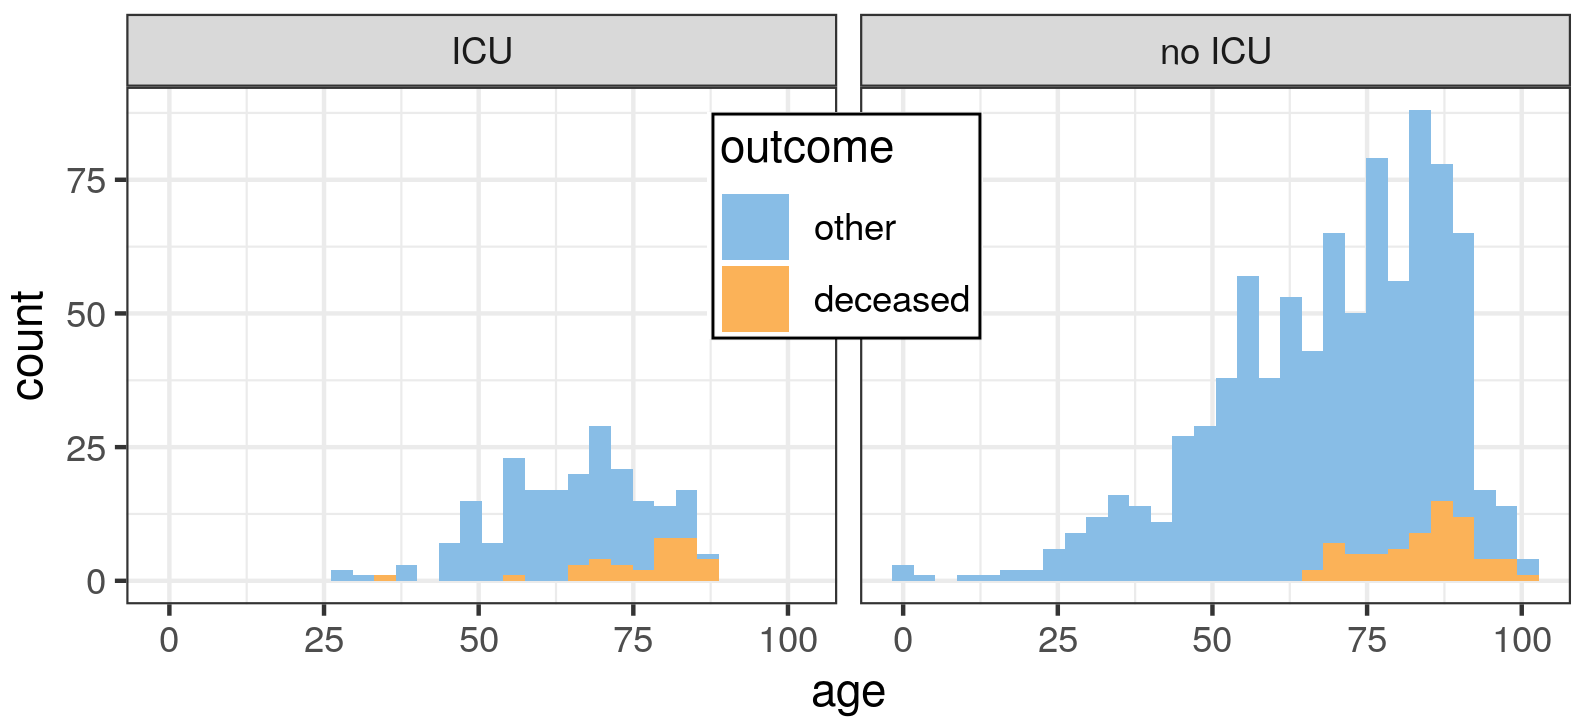
\includegraphics{fig_covid-switzerland-npi/fig_supp/VD_hist_age_mod.png}
    \label{fig:vdage}
\end{figure}
\begin{figure}[!htb]
    \centering
    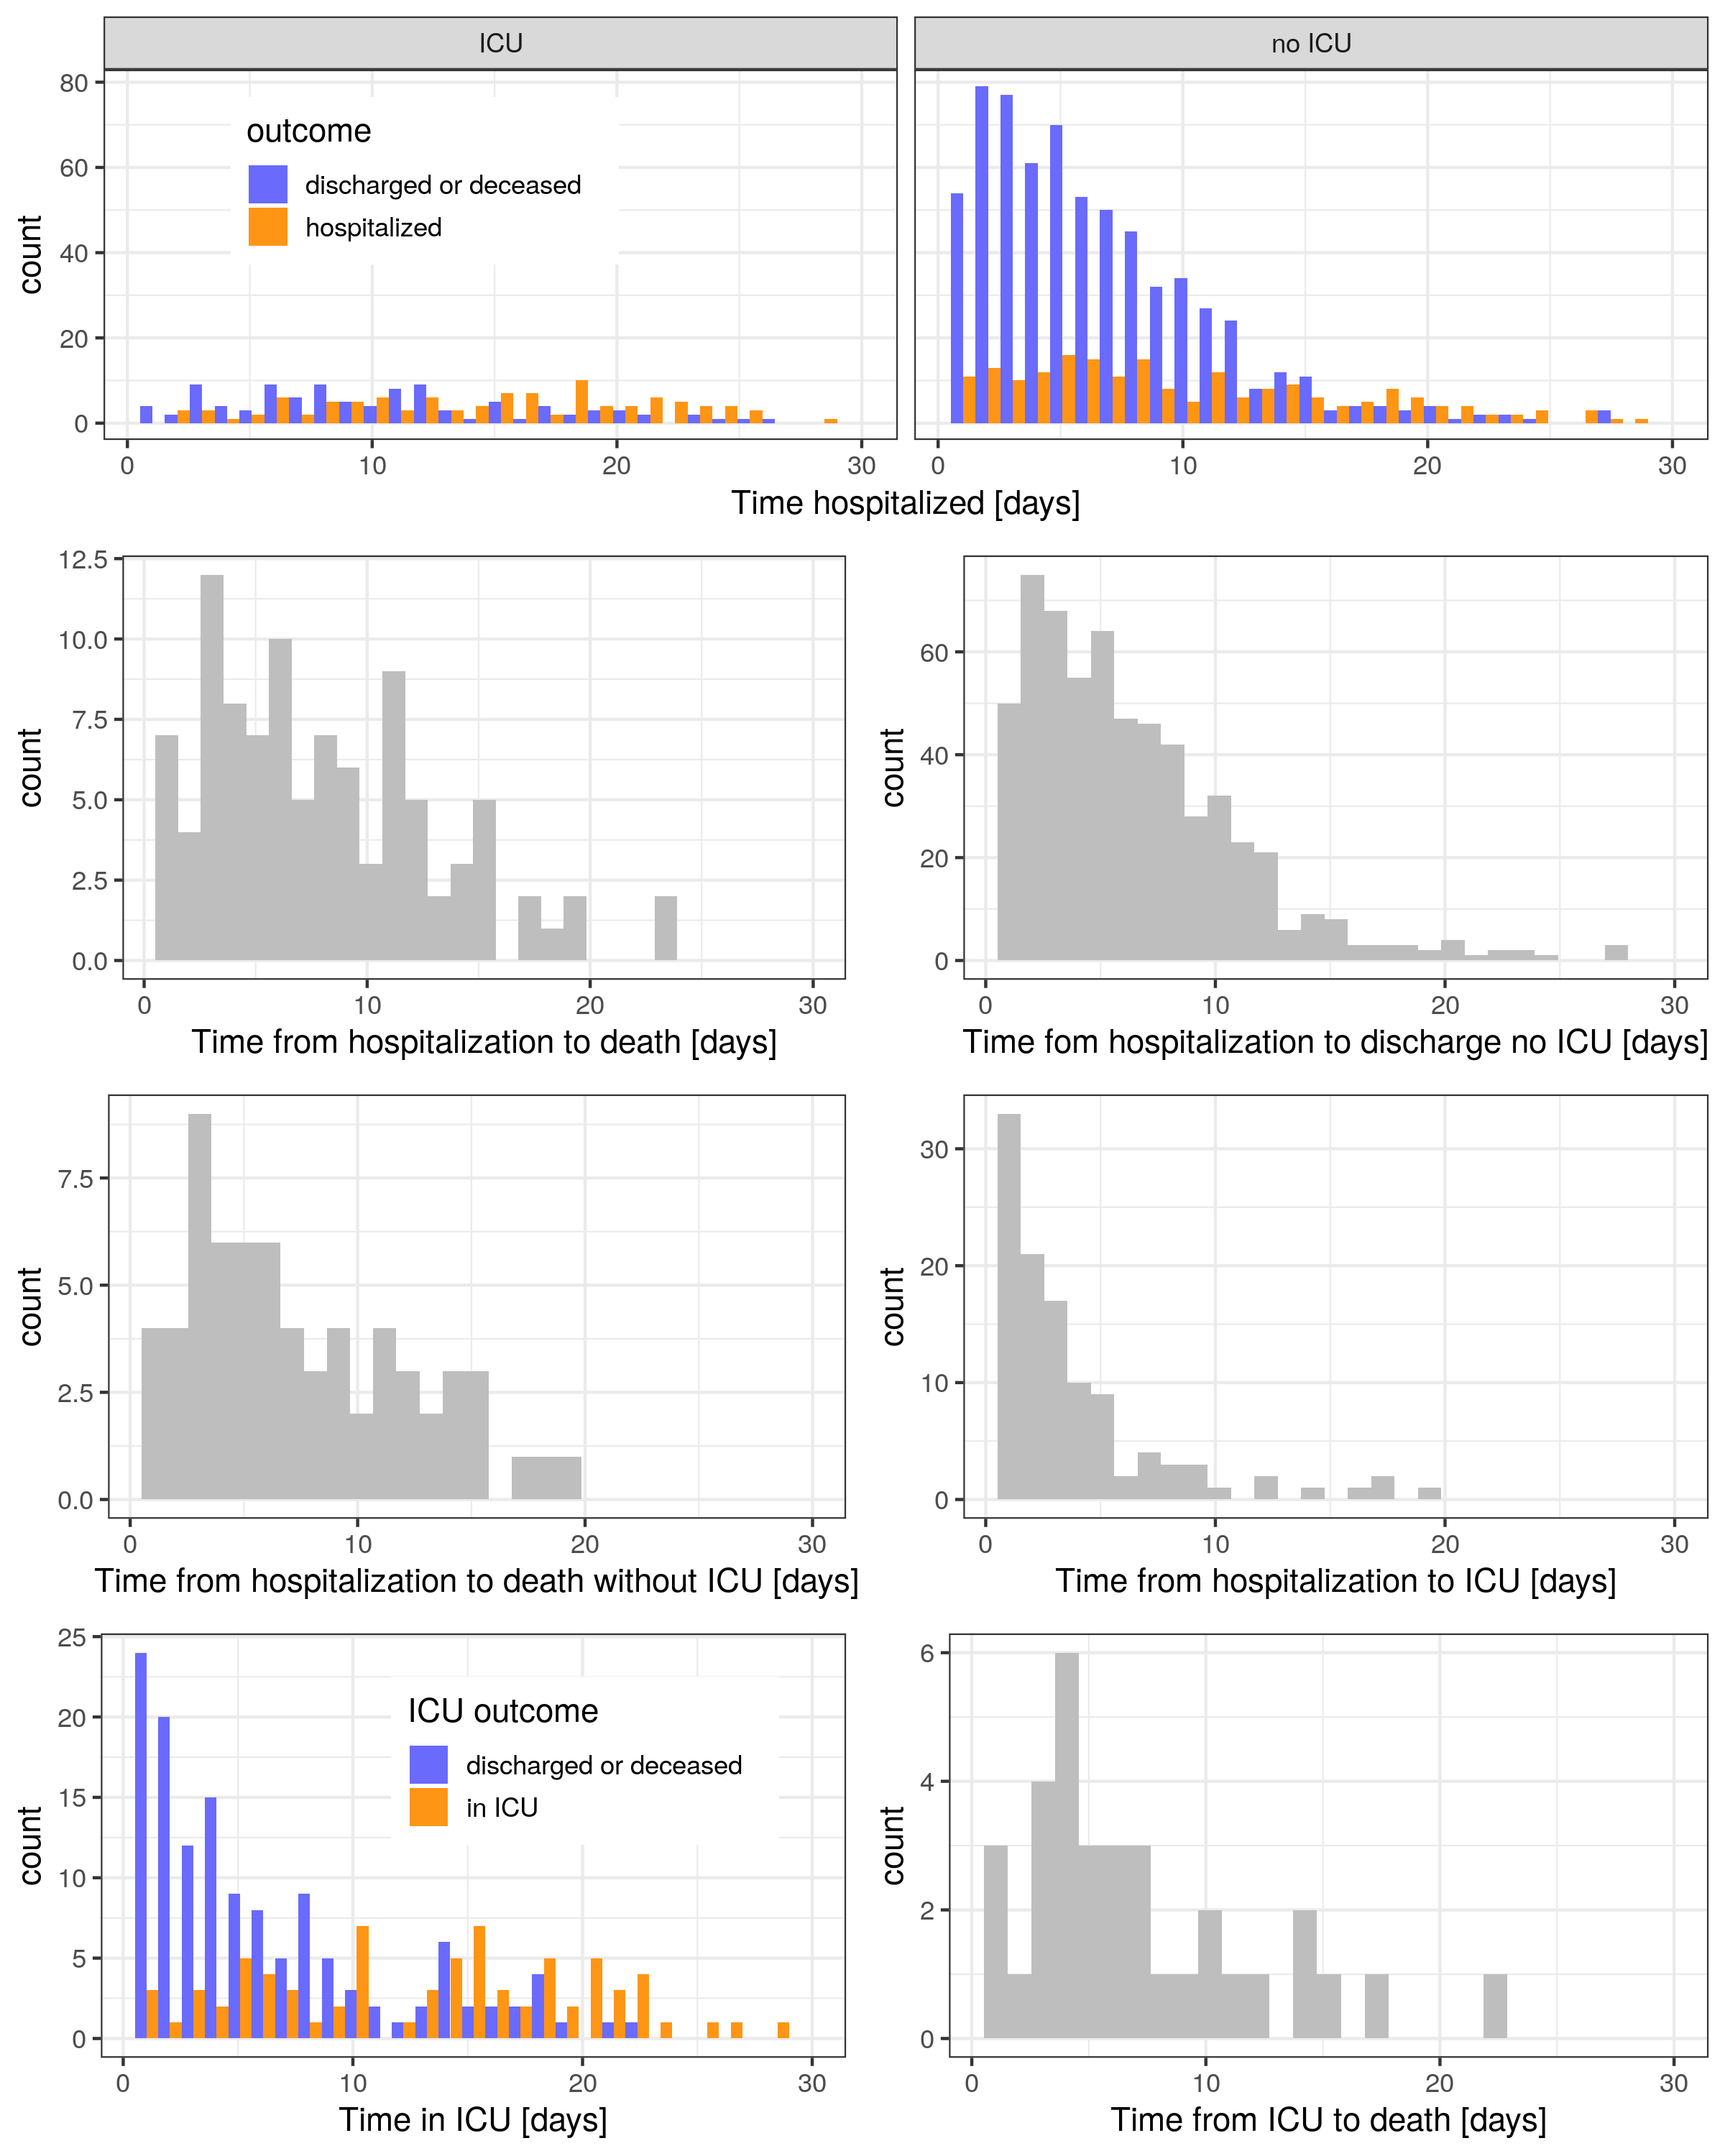
\includegraphics{fig_covid-switzerland-npi/fig_supp/VD_times.png}
    \caption[Key data of hospitalization events in canton de Vaud]{Data from canton de Vaud showing times to key hospitalization events. In order to perform this analysis, the patients are splitted in two categories: those who did not go through ICU during their stay and those who did. From left to right, top to bottom: total length of hospital stay for patients that went to ICU, then similarly for patient that did not. Then the time to death is shown for all patients, followed by both the time to discharge and to death for non-ICU patients. The last three graphs concerns ICU patients and detail ICU focused estimate: time from hospitalization to ICU, time in ICU and time from ICU to death. When meaningful, both currently hospitalized patient (orange) and already out-of-hospital patients (blue) are shown.}
    \label{fig:vdtimes}
\end{figure}

Of 777 patients with a known outcome on April 14, 104 died (13\%). The hospitalized Case Fatality Ratio (hCFR) is estimated by adjusting for the distribution of time hospitalization to death accounting for the fact that outcomes have not been yet observed for all patients (right-censoring\footnote[][-2\baselineskip]{The dataset presented here is two weeks more recent than the one visible in the example scenario planning report for Canton de Vaud (see Results, \textsc{Chapter 4}). It takes into account 137 additional patients, and the comparison with fig.~\ref{fig:vdage} strikingly shows how the distribution changes as the system is observed longer.}). To account for multiple outcomes (death and discharge), a parametric competing risk survival model is implemented\cite{Ghani:MethodsEstimatingCase:2005}. A Bayesian approach is choosen\cite{Bellot:TreebasedBayesianMixture:2018}, that enables us to fit parametric distributions to times to events using accelerated failure models. This method allows for the joint estimation of the probability of each event type and the distributions of times to events. In this case the probability of death, i.e. the hCFR. A \textsc{covid}-19 modeling study in France identified mixtures of probabilities of times to death, with a group dying faster with exponentially-distributed times and one dying slower\cite{Salje:EstimatingBurdenSARSCoV2:2020}. The Bayesian survival framework is extended to test for mixture in times to death and recovery. Model patients being discharged from ICU and subsequently dying, which was the case for 4/138 patients with known outcome, are not taken into account. Neither are accounted for multiple ICU stays per patient since this information was not available. Both Gamma and Log-Normal distributions are fitted separately to patients that did not go into ICU, and patients that did. For the former, it is modeled times from hospitalization to death or discharge, and for the latter times from ICU entry to both outcomes. Models were fit with Stan\cite[-5\baselineskip]{Carpenter:StanProbabilisticProgramming:2017}, and selection was done using Bayesian leave-one-out cross-validation\cite[-2.5\baselineskip]{Vehtari:PracticalBayesianModel:2017}. \\
\begin{figure}[!htb]
    \centering
        \caption[Survival functions of death and discharge for hospitalized patients and patients in ICU][-8\baselineskip]{Survival functions of death and discharge for hospitalized patients and patients in ICU. The lines represent the mean estimated cumulative probability of dying (full) and 1 minus the cumulative probability of discharge (dotted) estimated with non-parametric (Aalen-Johansen estimator, shading gives the 95\% CI) and parametric (assuming gamma and log-normal distributions, shading indicate the 95\% CrI) methods. Time is in days from hospitalization for patients that did not require ICU, and time from ICU admission for those that did. The point at which the lines join represents the probability that the final outcome is death, which was estimated to be 28.1\% (95\% CrI: 16.4-40.9) for patients in ICU and 13.0\% (95\% CrI: 9.9-16.6) for patients not requiring ICU based on the log-normal distribution.}
    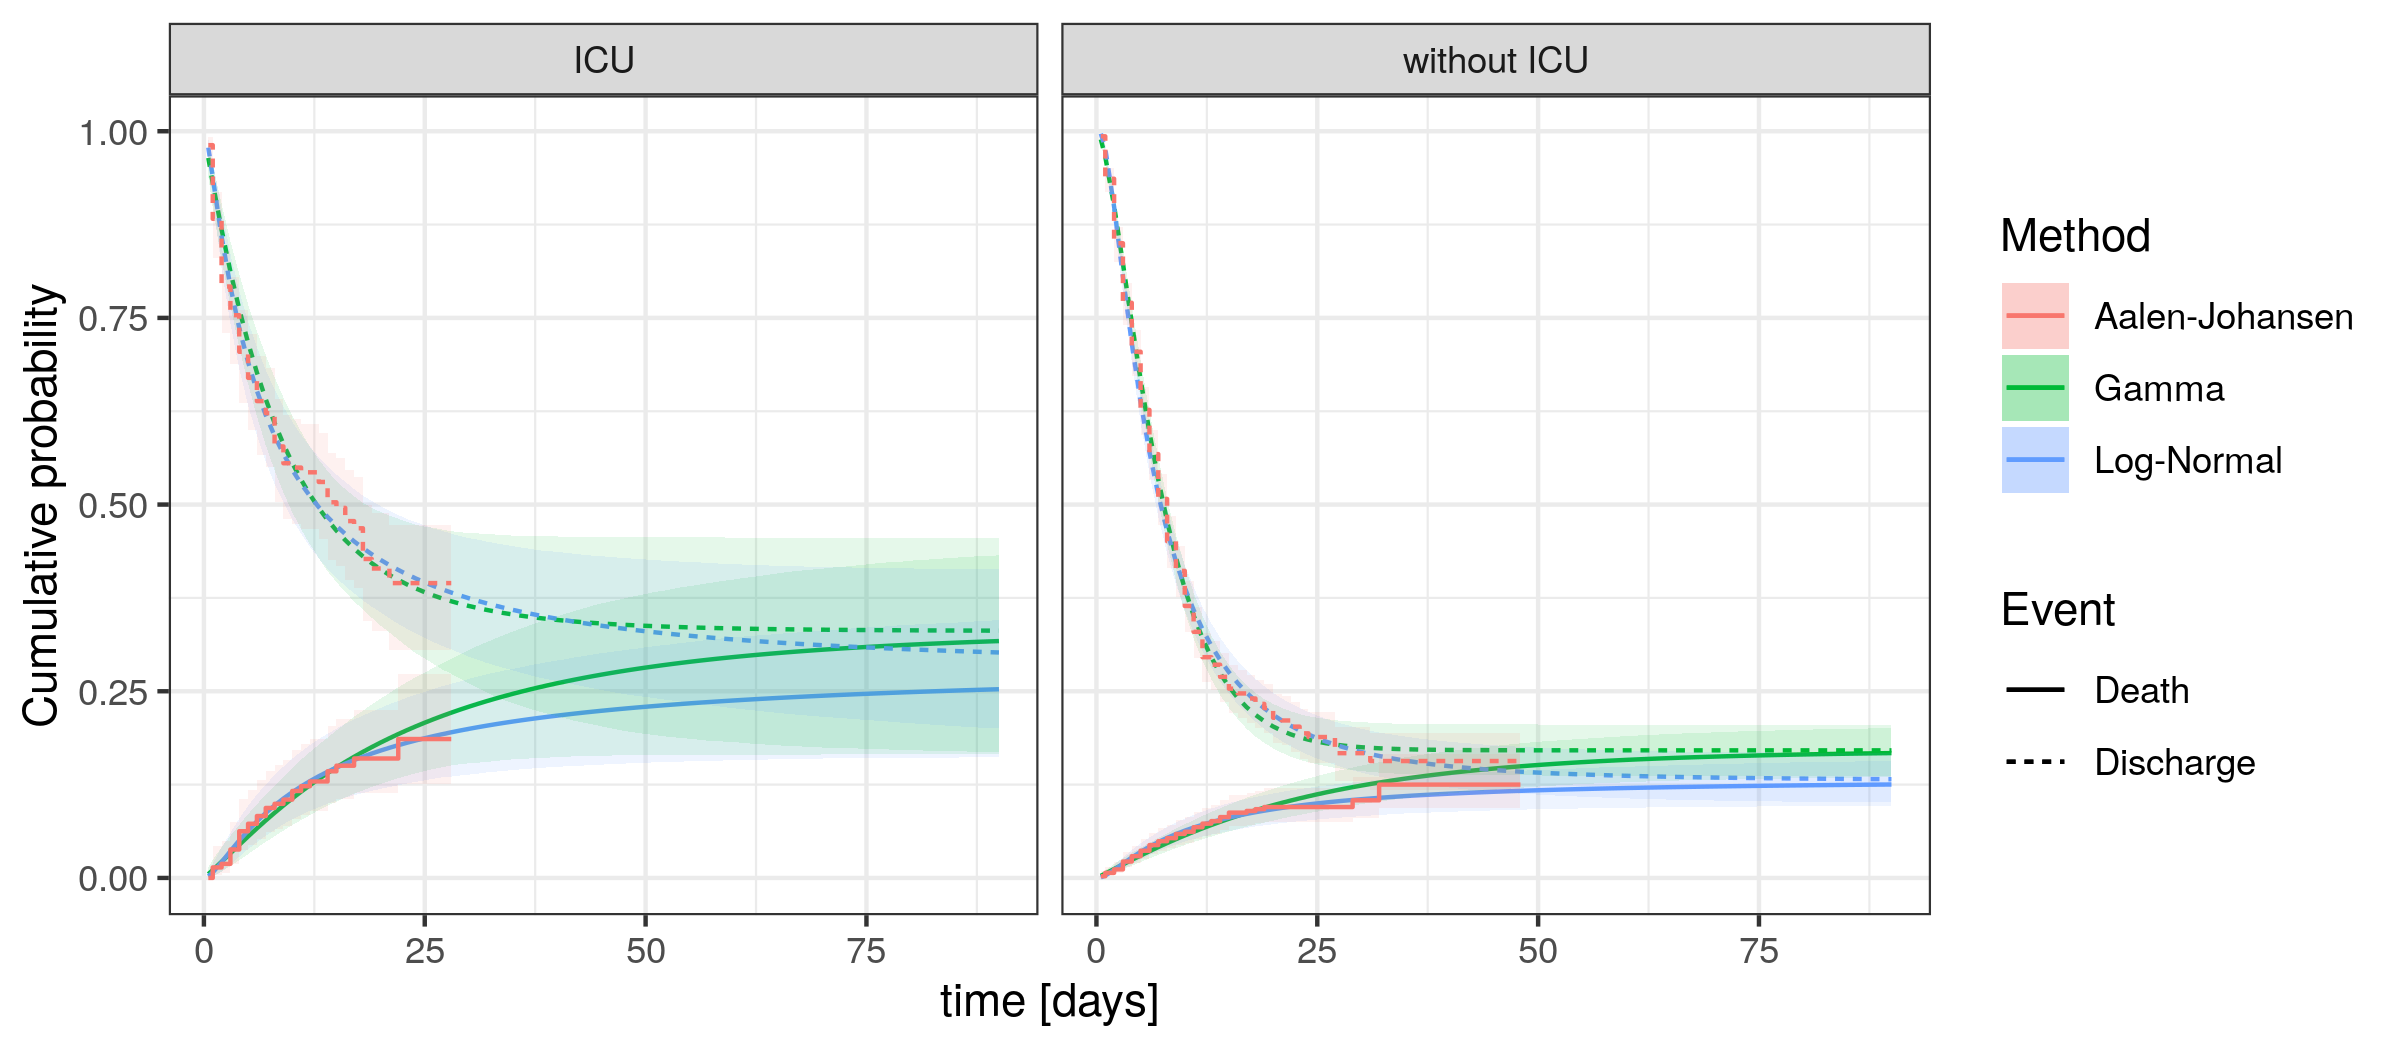
\includegraphics{fig_covid-switzerland-npi/fig_supp/survival_analaysis.png}
    \label{fig:delays}
\end{figure}


Times to death and discharge were best described by log-normal distributions with a single group both for patients having required ICU or not (fig.~\ref{fig:delays}). When accounting for right-censoring and assuming log-normally distributed times to events, an overall hCFR is estimated at 16.0\% (95\% credible interval, CrI: 12.5-19.8), resulting from a hCFR of 28.1\% (95\% CrI: 16.4-40.9) for patients requiring ICU and 13.0\% (95\% CrI: 9.9-16.6) for patients that did no require it. Estimated hCFRs were slightly higher when assuming gamma-distributed times to events (overall hCFR of 20.3\%, 95\% CrI: 15.9-24.1). The distribution of times of hospitalization processes are shown in fig.~\ref{fig:vdtimes}, and fitted distribution parameters given in tab.~\ref{tab:vdparams}.

\begin{table}[t]
\caption[Observed hospitalization time distributions]{Observed hospitalization time distributions. All times are in days and taken from the date of hospitalization if not specified otherwise. Note that these estimates are biased due to right-censoring of observations and probably under-estimate the true distributions. Estimates that account for right-censoring are shown in tab.~\ref{tab:survpars}.}
\label{tab:vdparams}
\centering
\begin{tabular}{lrrrr}
\toprule
 & mean & sd & mean (logscale) & sd (logscale)\\
\midrule
Time hospitalized & 8.49 & 6.58 & 1.81 & 0.87\\
Time to death & 8.23 & 6.09 & 1.80 & 0.87\\ \addlinespace
Time to discharge without ICU & 6.29 & 4.66 & 1.56 & 0.80\\
Time hospitalized without ICU & 7.35 & 5.79 & 1.68 & 0.85\\
Time to death without ICU & 7.84 & 6.27 & 1.73 & 0.88\\ \addlinespace
Time to ICU & 2.35 & 3.79 & 0.18 & 1.05\\
Time hospitalized with ICU & 13.14 & 7.50 & 2.37 & 0.72\\
Time in ICU & 8.36 & 6.76 & 1.69 & 1.04\\
Time from ICU to discharge & 8.68 & 6.99 & 1.71 & 1.07\\
Time from ICU to death & 6.97 & 4.98 & 1.68 & 0.77\\
\bottomrule
\end{tabular}
\end{table}


\begin{fwtable}
    \centering
    \begin{tabular}{ccccccc}
\toprule
 & & \multicolumn{3}{c}{Log-Normal} & \multicolumn{2}{c}{Gamma}\\ \cmidrule(rl){3-5} \cmidrule(rl){6-7}
Group & Event & median & mean-log & SD-log & scale & shape\\
\midrule
Without ICU & Death & 10 (7.3--16) & 2.3 (2--2.8) & 1.2 (0.95--1.5) & 21 (21--22) & 1.1 (0.83--1.4)\\
 & Discharge & 6.1 (5.6--6.6) & 1.8 (1.7--1.9) & 0.93 (0.87--0.99) & 4.3 (4.4--4.2) & 1.8 (1.6--2)\\ \addlinespace
ICU & Death & 13 (6.2--30) & 2.6 (1.8--3.4) & 1.3 (0.87--1.9) & 21 (12--23) & 1.2 (0.74--1.9)\\
 & Discharge & 6.4 (4.3--9.3) & 1.8 (1.5--2.2) & 1.3 (1.1--1.6) & 9.1 (8.1--11) & 1 (0.75--1.4)\\
\bottomrule
\end{tabular}
\caption[Estimated parameters of hospitalization time distributions]{Estimated parameters of hospitalization time distributions. These estimates differ from observed values given in tab.~\ref{tab:vdparams} by accounting for right-censoring of observations. Time from hospitalization to discharge or death, and from ICU admission to discharge or death are reported here. Estimates were obtained using competing risk survival model as described above. Parameters are given in terms of their posterior mean and 95\% CrI (in parenthesis). For the log-normal distribution the parameters correspond to the mean and SD of the logarithm of the distribution.}
     \label{tab:survpars}
\end{fwtable}

%We build a \textsc{covid}-19 compartmental transmission model based on the Susceptible Exposed Infected Recovered (SEIR) template with three I compartments. The schematic with the different transitions and compartments is shown in SM Fig.~\ref{fig:diagram}. Infected individuals have some probability of developing severe symptoms which require hospitalization after a delay from symptom onset ($I_h$). Hospitalization can lead to recovery or death, either through normal hospitalization ($H_{s}$ and $H_d$ respectively) or passing through Intensive Care Units (ICUs) ($U_{s}$ and $U_d$ respectively). Data from the canton of Vaud show a high proportion of deaths outside of hospitals ($\approx 50\%$), we therefore also include a pathway from infection to death without passing through hospitalization ($I_d$). 


%The time spent in the observable hospitalization states were used to define the number of stages in each compartment by fitting Erlang distributions to the data of canton de Vaud. To account for right-censoring we do not fit directly to observed times to events but rather to the estimated log-normal distributions described in the survival analysis section above. We fit the rate parameter of the Erlang distributions for shape parameters between 1 and 10 by minimizing the Kullback-Leibler (KL) divergence between the Erlang and estimated log-normal distributions. The final fit was taken to be the one with the smallest KL-divergence. \\


%\section{Model equations}\label{sec:stoch}
%As in \textsc{Chapter 2} and 3, the model is implemented as a discrete-state model based on a Partially-Observed Markov Process (POMP), or equivalently a Hidden Markov Model (HMM), simulating the transitions between compartments as discrete events using stochastic count processes\cite{King:InapparentInfectionsCholera:2008,Breto:TimeSeriesAnalysis:2009}. Let \(N_{AB}(t)\) be the number of individuals transiting between compartments \(A,B\in \mathcal{X}\) in the time interval \([0,t)\)  where $\mathcal{X}$ is the state vector,
%$$\mathcal{X} = \{S, E, I_{1,2,3} , I_d, I_h, H_{s}, H_{d}, H_{u}, U_{s}, U_{d}, R, D\}$$
%
%Using the same notation as previous chapters, the number of transitions during a time-step $\Delta t$ is
%\(\Delta N_{AB}(t) = N_{AB}(t+\Delta t) - N_{AB}(t)\). We model time-varying $R_0(t) = \beta(t)/(3r_I)$ as a geometric random walk defined by its calibrated variance, where $\beta$ is the transmission parameter and $1/(3r_I)$ is the mean duration spent in the infectious compartments $I_1$ to $I_3$. The force of infection is expressed in terms of $\beta(t)$ in the model. Given the state of the system at time \(t\), \(\mathcal{X}_t\), the model reads:
%\begin{gather}
%\label{eq:stochsys}
%\begin{aligned}
%    \mathbb{P}\left[ \Delta N_{SE}(t) = 1 \right|\mathcal{X}_t] &=  \beta(t)  \frac{I_1(t) + I_2(t) + I_3(t)}{P} S(t) \Delta t + o(\Delta t)\\
%    \mathbb{P}\left[ \Delta N_{EI_1}(t) = 1 \right|\mathcal{X}_t] &= r_{E} E(t) \Delta t + o(\Delta t) \\
%    \mathbb{P}\left[ \Delta N_{I_1 I_2}(t) = 1 \right|\mathcal{X}_t] &= 3r_{I} I_1(t) \Delta t + o(\Delta t)\\
%    \mathbb{P}\left[ \Delta N_{I_2 I_3}(t) = 1 \right|\mathcal{X}_t] &= 3r_{I} I_2(t) \Delta t + o(\Delta t)\\
%    \mathbb{P}\left[ \Delta N_{I_3 I_d}(t) = 1 \right|\mathcal{X}_t] &= p_{I_d|I_3} \cdot 3r_{I}  I_3(t) \Delta t + o(\Delta t)\\
%    \mathbb{P}\left[ \Delta N_{I_3 I_h}(t) = 1 \right|\mathcal{X}_t] &= p_{I_h|I_3} \cdot 3r_{I}   I_3(t) \Delta t + o(\Delta t)\\
%    \mathbb{P}\left[ \Delta N_{I_3 R}(t) = 1 \right|\mathcal{X}_t] &= p_{R|I_3} \cdot 3r_{I}  I_3(t) \Delta t + o(\Delta t)\\
%    \mathbb{P}\left[ \Delta N_{I_d R}(t) = 1 \right|\mathcal{X}_t] &= p_{R|I_d} \cdot r_{I}  I_d(t) \Delta t + o(\Delta t)\\
%    \mathbb{P}\left[ \Delta N_{I_d D}(t) = 1 \right|\mathcal{X}_t] &= p_{D|I_d}\cdot r_{I} I_d(t) \Delta t + o(\Delta t)\\
%    \mathbb{P}\left[ \Delta N_{I_h H_d}(t) = 1 \right|\mathcal{X}_t] &= p_{H_d|I_h} \cdot r_{I_h}  I_h(t) \Delta t + o(\Delta t)\\
%    \mathbb{P}\left[ \Delta N_{I_h H_u}(t) = 1 \right|\mathcal{X}_t] &= p_{H_u|I_h} \cdot r_{I_h} I_h(t) \Delta t + o(\Delta t)\\
%    \mathbb{P}\left[ \Delta N_{I_h H_s}(t) = 1 \right|\mathcal{X}_t] &= p_{H_s|I_h} \cdot r_{I_h} I_h(t) \Delta t + o(\Delta t)\\
%   \mathbb{P}\left[ \Delta N_{H_s R}(t) = 1 \right|\mathcal{X}_t] &=  r_{H_s} H_s(t) \Delta t + o(\Delta t)\\
%    \mathbb{P}\left[ \Delta N_{H_u U_d}(t) = 1 \right|\mathcal{X}_t] &=   p_{U_d|H_u} \cdot r_{H_u} H_u(t) \Delta t + o(\Delta t)\\
%    \mathbb{P}\left[ \Delta N_{H_u U_s}(t) = 1 \right|\mathcal{X}_t] &=   p_{U_s|H_u} \cdot r_{H_u} H_u(t) \Delta t + o(\Delta t)\\
%    \mathbb{P}\left[ \Delta N_{H_d D}(t) = 1 \right|\mathcal{X}_t] &=   r_{H_d} H_d(t) \Delta t + o(\Delta t)\\
%    \mathbb{P}\left[ \Delta N_{U_s R}(t) = 1 \right|\mathcal{X}_t] &=   r_{U_s} U_s(t) \Delta t + o(\Delta t)\\
%    \mathbb{P}\left[ \Delta N_{U_d D}(t) = 1 \right|\mathcal{X}_t] &=   r_{U_d} U_d(t) \Delta t + o(\Delta t)\\
%\end{aligned}
%\end{gather}
%
%\noindent assuming that \(\mathbb{P}[\Delta N_{XY} > 1|\mathcal{X}_t] = o(\Delta t) \; \forall X,Y \in \mathcal{X}\). Branching probabilities from stage $X$ to $Y$ are noted $p_{Y|X}$ and rates of stay in stage $X$ is noted $r_X$.
%The ensuing stochastic variations of the state variables are:
%\begin{gather}
%\label{eq:stochstates}
%\begin{aligned}
%    \Delta E(t) &= \Delta N_{SE}(t) - \Delta N_{EI_1}(t))\\
%    \Delta I_1(t) &= \Delta N_{EI_1}(t) - \Delta N_{I_1 I_2}\\
%    \Delta I_2(t) &= \Delta N_{I_1 I_2} - \Delta N_{I_2 I_3}\\
%    \Delta I_3(t) &=  \Delta N_{I_2 I_3} - \Delta N_{I_3 I_d} - \Delta N_{I_3 I_h} -  \Delta N_{I_3 R}\\
%    \Delta I_d(t) &= \Delta N_{I_3 I_d} - \Delta N_{I^d R} - \Delta N_{I^d D}\\
%    \Delta I_h(t) &= \Delta N_{I_3 I_h} -  \Delta N_{I_h H_d} -  \Delta N_{I_h H_u} -  \Delta N_{I_h H_s} \\
%    \Delta H_s(t) &= \Delta N_{I_h H_s} -  \Delta N_{H_s R}\\
%   \Delta H_d(t) &= \Delta N_{H_s H_d} -  \Delta N_{H_d D}\\
%    \Delta H_u(t) &= \Delta N_{I_h H_u} - \Delta N_{H_u U_d} - \Delta N_{H_u U_a} - \Delta N_{H_u U}\\
%    \Delta U(t) &=  \Delta N_{H_u U} - \Delta N_{U R}\\
%    \Delta U_d(t) &=  \Delta N_{H_u U_d} - \Delta N_{U_d D}\\
%    \Delta D(t) &=  \Delta N_{I^d D} + \Delta N_{U_d D} + \Delta N_{H_d D}\\
%    \Delta R(t) &= \Delta N_{I_3 R} + \Delta N_{I^d R} +  \Delta N_{H_s R} + \Delta N_{U R} \\
%     S(t) &= P - \sum_{X \in \mathcal{X} \backslash \{S\}} X(t),
%\end{aligned}
%\end{gather}
%where the equation for \(S(t)\) enforces a constant total population. The total population for each canton and for Switzerland is taken from the 2018 estimate of the Federal Statistical Office\cite{Officefederaldelastatistique:Population:2018}.
%
%
%\section{Model Parameters}
%Rates of transitions are shown Table~\ref{parRates} and branching probabilities in Table~\ref{parProb}. Proper indentifiability is needed to capture the dynamics of $R_0$ so most of the parameters where fixed to values of the litterature.
%The model is parameterized conditioning on a mean generation time of 5.2 days \parencite{Ganyani:EstimatingGenerationInterval:2020}, and an exposed and non-infectious duration of 2.9 days \parencite{He:TemporalDynamicsViral:2020}, yielding a mean duration of 4.6 days in the infectious compartments. All rates are given in day$^{-1}$ and the subscript subscript in the parameter names indicate the compartment from which exits happen at the given rate.
%
%
%\begin{table*}[ht!]
%\centering\small
%\begin{tabular}{lccl} 
%\toprule
%Rate & Source & Value or starting bound & Corresponding duration  \\
%\midrule
%$r_{E}$ & \parencite{He:TemporalDynamicsViral:2020} & $1/2.9$& infected but non-infectious state \\
%$r_{I}$ & \parencite{He:TemporalDynamicsViral:2020, Ganyani:EstimatingGenerationInterval:2020}  & $1/4.6$  & infectious state\\
%$r_{I_h}$ & \parencite{Scire:ReproductiveNumberCOVID19:2020} & $1/1.6$& end of the infectious period to hospitalization \\
%$r_{H_s}$ & Vaud data & $1/7.6$ & hospitalization to discharge \\
%$r_{H_d}$ & Vaud data & $1/23.7$ & hospitalization to death \\
%$r_{H_u}$ & Vaud data & $1/2.35$  & hospitalization to ICU admission \\
%$r_{U_s}$ & Vaud data & $1/9.3$  & ICU admission to discharge \\
%$r_{U_d}$ & Vaud data & $1/25.6$ & ICU admission to death \\
%$r_{I_d}$ & Fitted & $1/50 - 1/1$ &end of the infectious period to death when not hospitalized \\
%\bottomrule
%\end{tabular}
%\caption[Transition rates from each compartment of the model]{Transition rates from each compartment of the model. Compartments $I_{1,2,3}$ are composed of several stages so the rate of exit from each one is $3r_{I}$. }
%\label{parRates}
%\end{table*}
%
%There are seven different pathways from susceptible to either death or recovery. It is assumed that the proportion of severe infections that have severe symptoms which would require hospitalization is of 7.5\% \parencite{Verity:EstimatesSeverityCoronavirus:2020}, that 50\% of deaths happen outside of hospitals (data from cantons of Vaud as above and Geneva from OpenZH), that the hospitalized case fatality ratio is of 16\% (data from canton of Vaud, see above), the probability of going into ICU for hospitalized patients is of 20\% (data from canton of Vaud), and an population-level infection fatality ratio (IFR) of 0.75 \% which is in the range of published estimates\parencite{Verity:EstimatesSeverityCoronavirus:2020,Russell:EstimatingInfectionCase:2020}.
%\begin{table*}[ht!]
%\centering\small
%\begin{tabular}{lccl} 
%\toprule
%Parameter & Source & Value &  Description \\
%\midrule
%IFR & Assumed & 0.0075 & Infection fatality ratio \\
%$p_s$ & Assumed &  0.075 & Probability of severe symptoms\\
%$p_h$ &  Vaud data $|$ IFR &  0.31 & Probability of hospitalization given severe symptoms  \\
%$p_{I_d|I_3}$ & Vaud data $|$ IFR, $p_s$ & $p_s (1-p_h)$&  Probability of death outside of the hospital given sever symptoms  \\
%$p_{I_h|I_3}$ & Vaud data $|$ IFR, $p_s$  & $p_s p_h$   &  Probability of hospitalization given infection \\
%$p_{R|I_3}$   & Deduced  $|p_s$ & $(1-p_s)$    &  Probability of not having sever symptoms\\
%$p_{D|I_d}$   & Vaud data $|$ IFR, $p_s$  &  0.073   &  Probability of death given severe symptoms and not hospitalized \\
%$p_{R|I_d}$   & Vaud data $|$ IFR, $p_s$ &  $1-p_{D|I_d}$   & Probabilitys of recovery given severe symptoms \\
%$p_{H_s|I_h}$ & Vaud data &  0.72   &  probability of discharge without ICU given hospitalization\\
%$p_{H_d|I_h}$ & Vaud data &  0.11    &  Probability of death given not going into ICU\\
%$p_{H_u|I_h, !H_s}$ & Vaud data &  0.61   &  Probability of ICU given not discharged without ICU\\
%$p_{U_d|H_u}$ & Vaud data & 0.28   &  Probability of death given ICU \\
%\bottomrule
%\end{tabular}
%\caption[Branching probabilities of the model]{Branching probabilities of the model. The probability of transition from stage $A$ to stage $B$ is $p_{B|A}$. }
%\label{parProb}
%\end{table*}
%
%
%\section{Assessment of Model Fit}
%In fig. \ref{fig:chfit} and fig. \ref{fig:cantonfit}, model fits at respectively the national and cantonal levels are showed. Note that the hospitalization processes in all cantons and at the national level were parameterized with data from the canton de Vaud. Difference in hospital protocols and procedures in each canton as well as transfers of patient between cantons cause differences between observed and modelled ICU occupancy. This model tends to overestimate current ICU using time distributions from canton de Vaud, while death (cumulative and incidence) and current hospitalization are well captured. 
% 
%\begin{figure}[!htb]
%    \centering
%    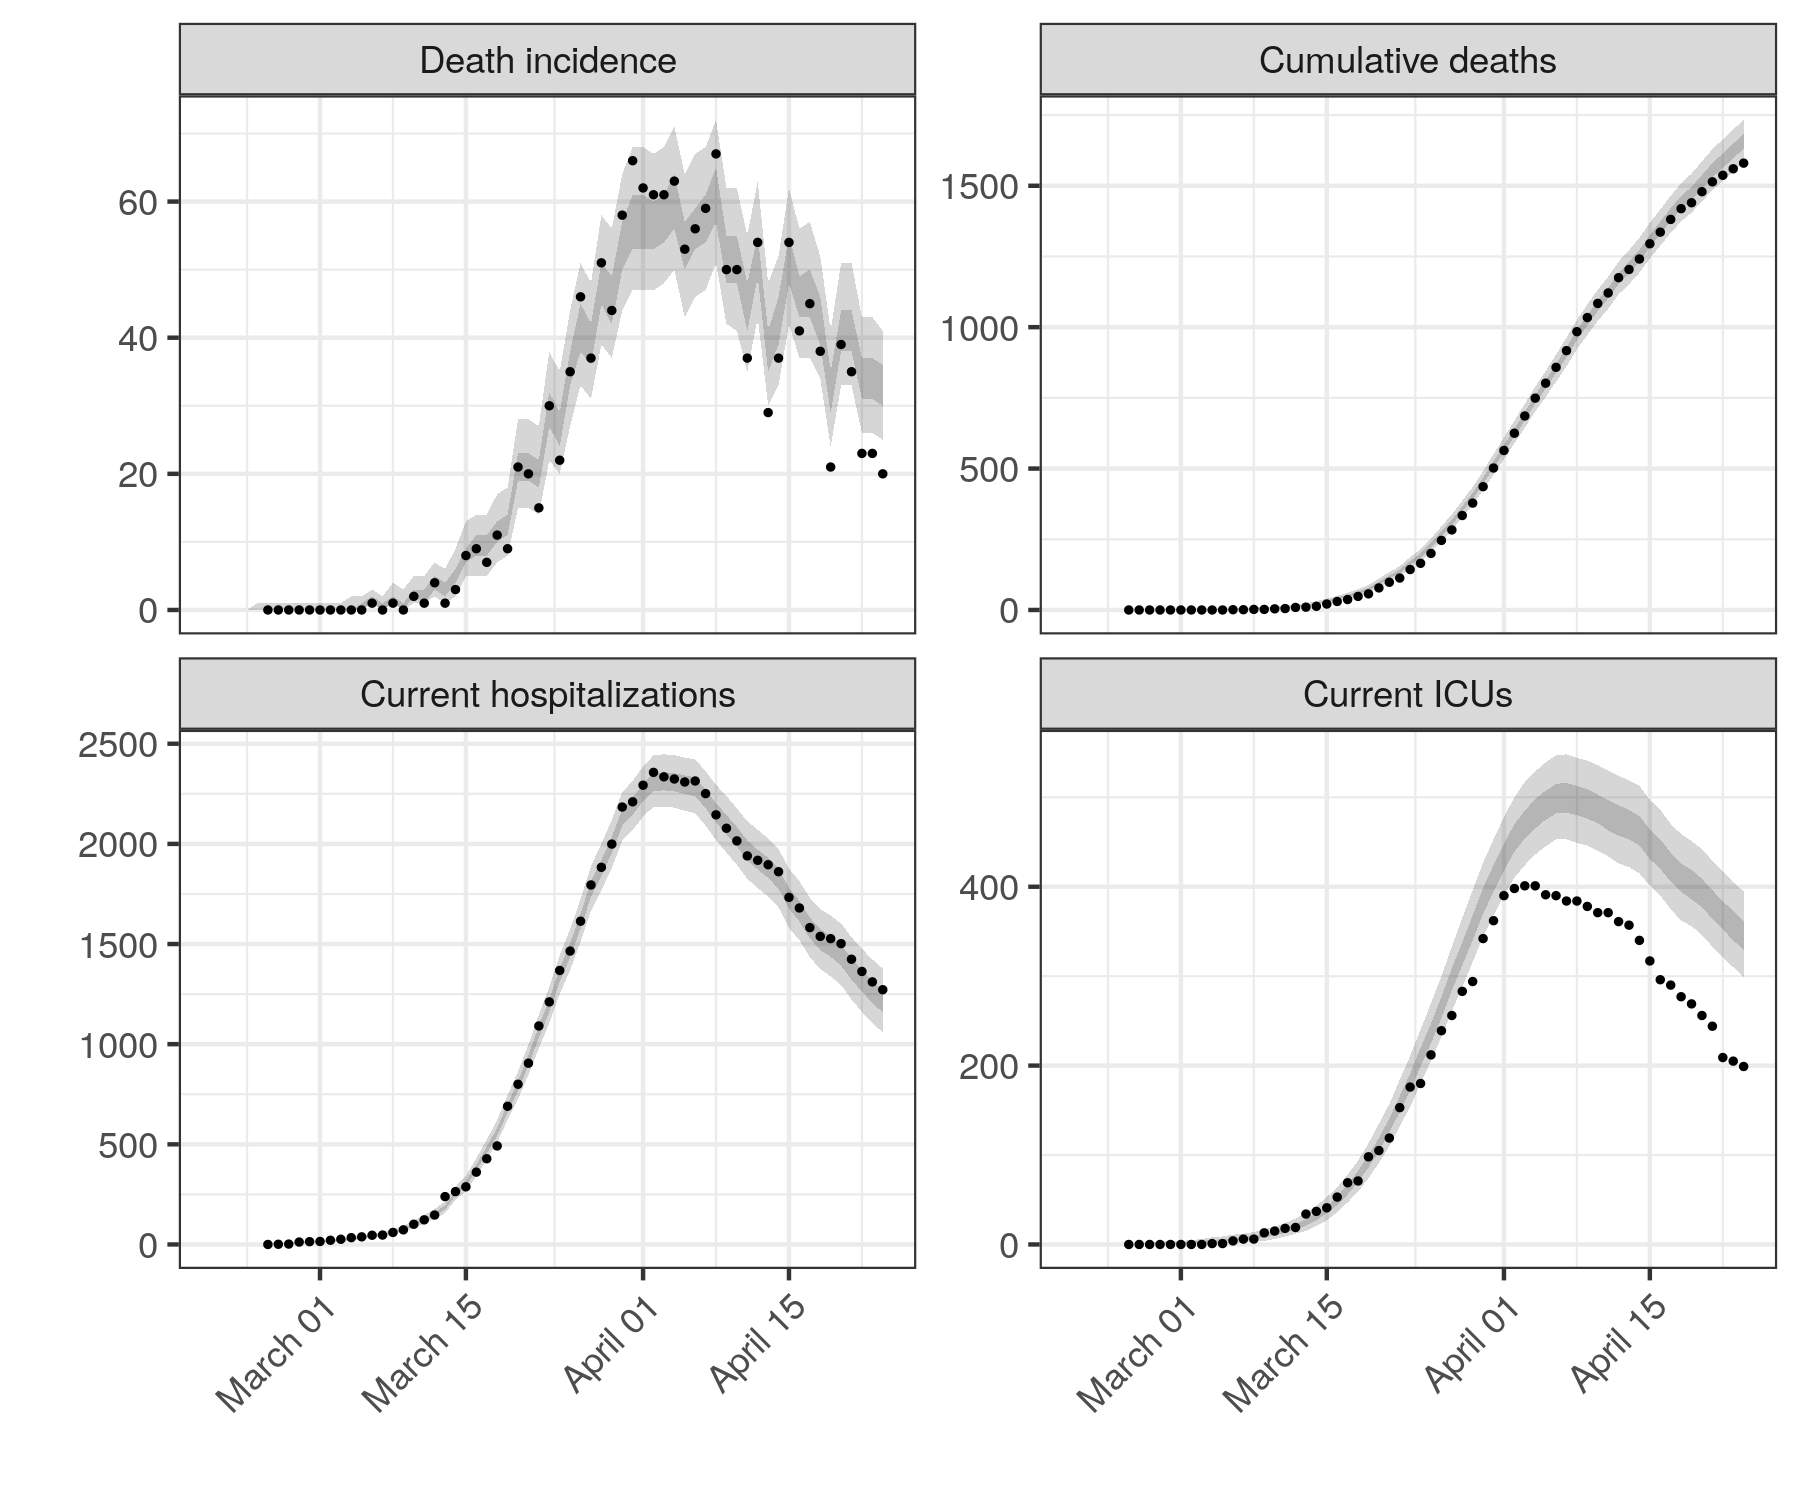
\includegraphics{fig_covid-switzerland-npi/fig_supp/CH_fits.png}
%    \caption[Model fit at at national level]{Model fit at at national level. Model results are given in terms of the 95\% (light gray) and 50\% quantile ranges of the smoothing distribution of R$_0$ at the maximum likelihood estimates of inferred parameters. Data (points) from \textcite{Probst:DaenuprobstCovid19casesswitzerland:2020}}.     \label{fig:chfit}
%\end{figure}
%
%\begin{figure}[!htb]
%    \centering
%    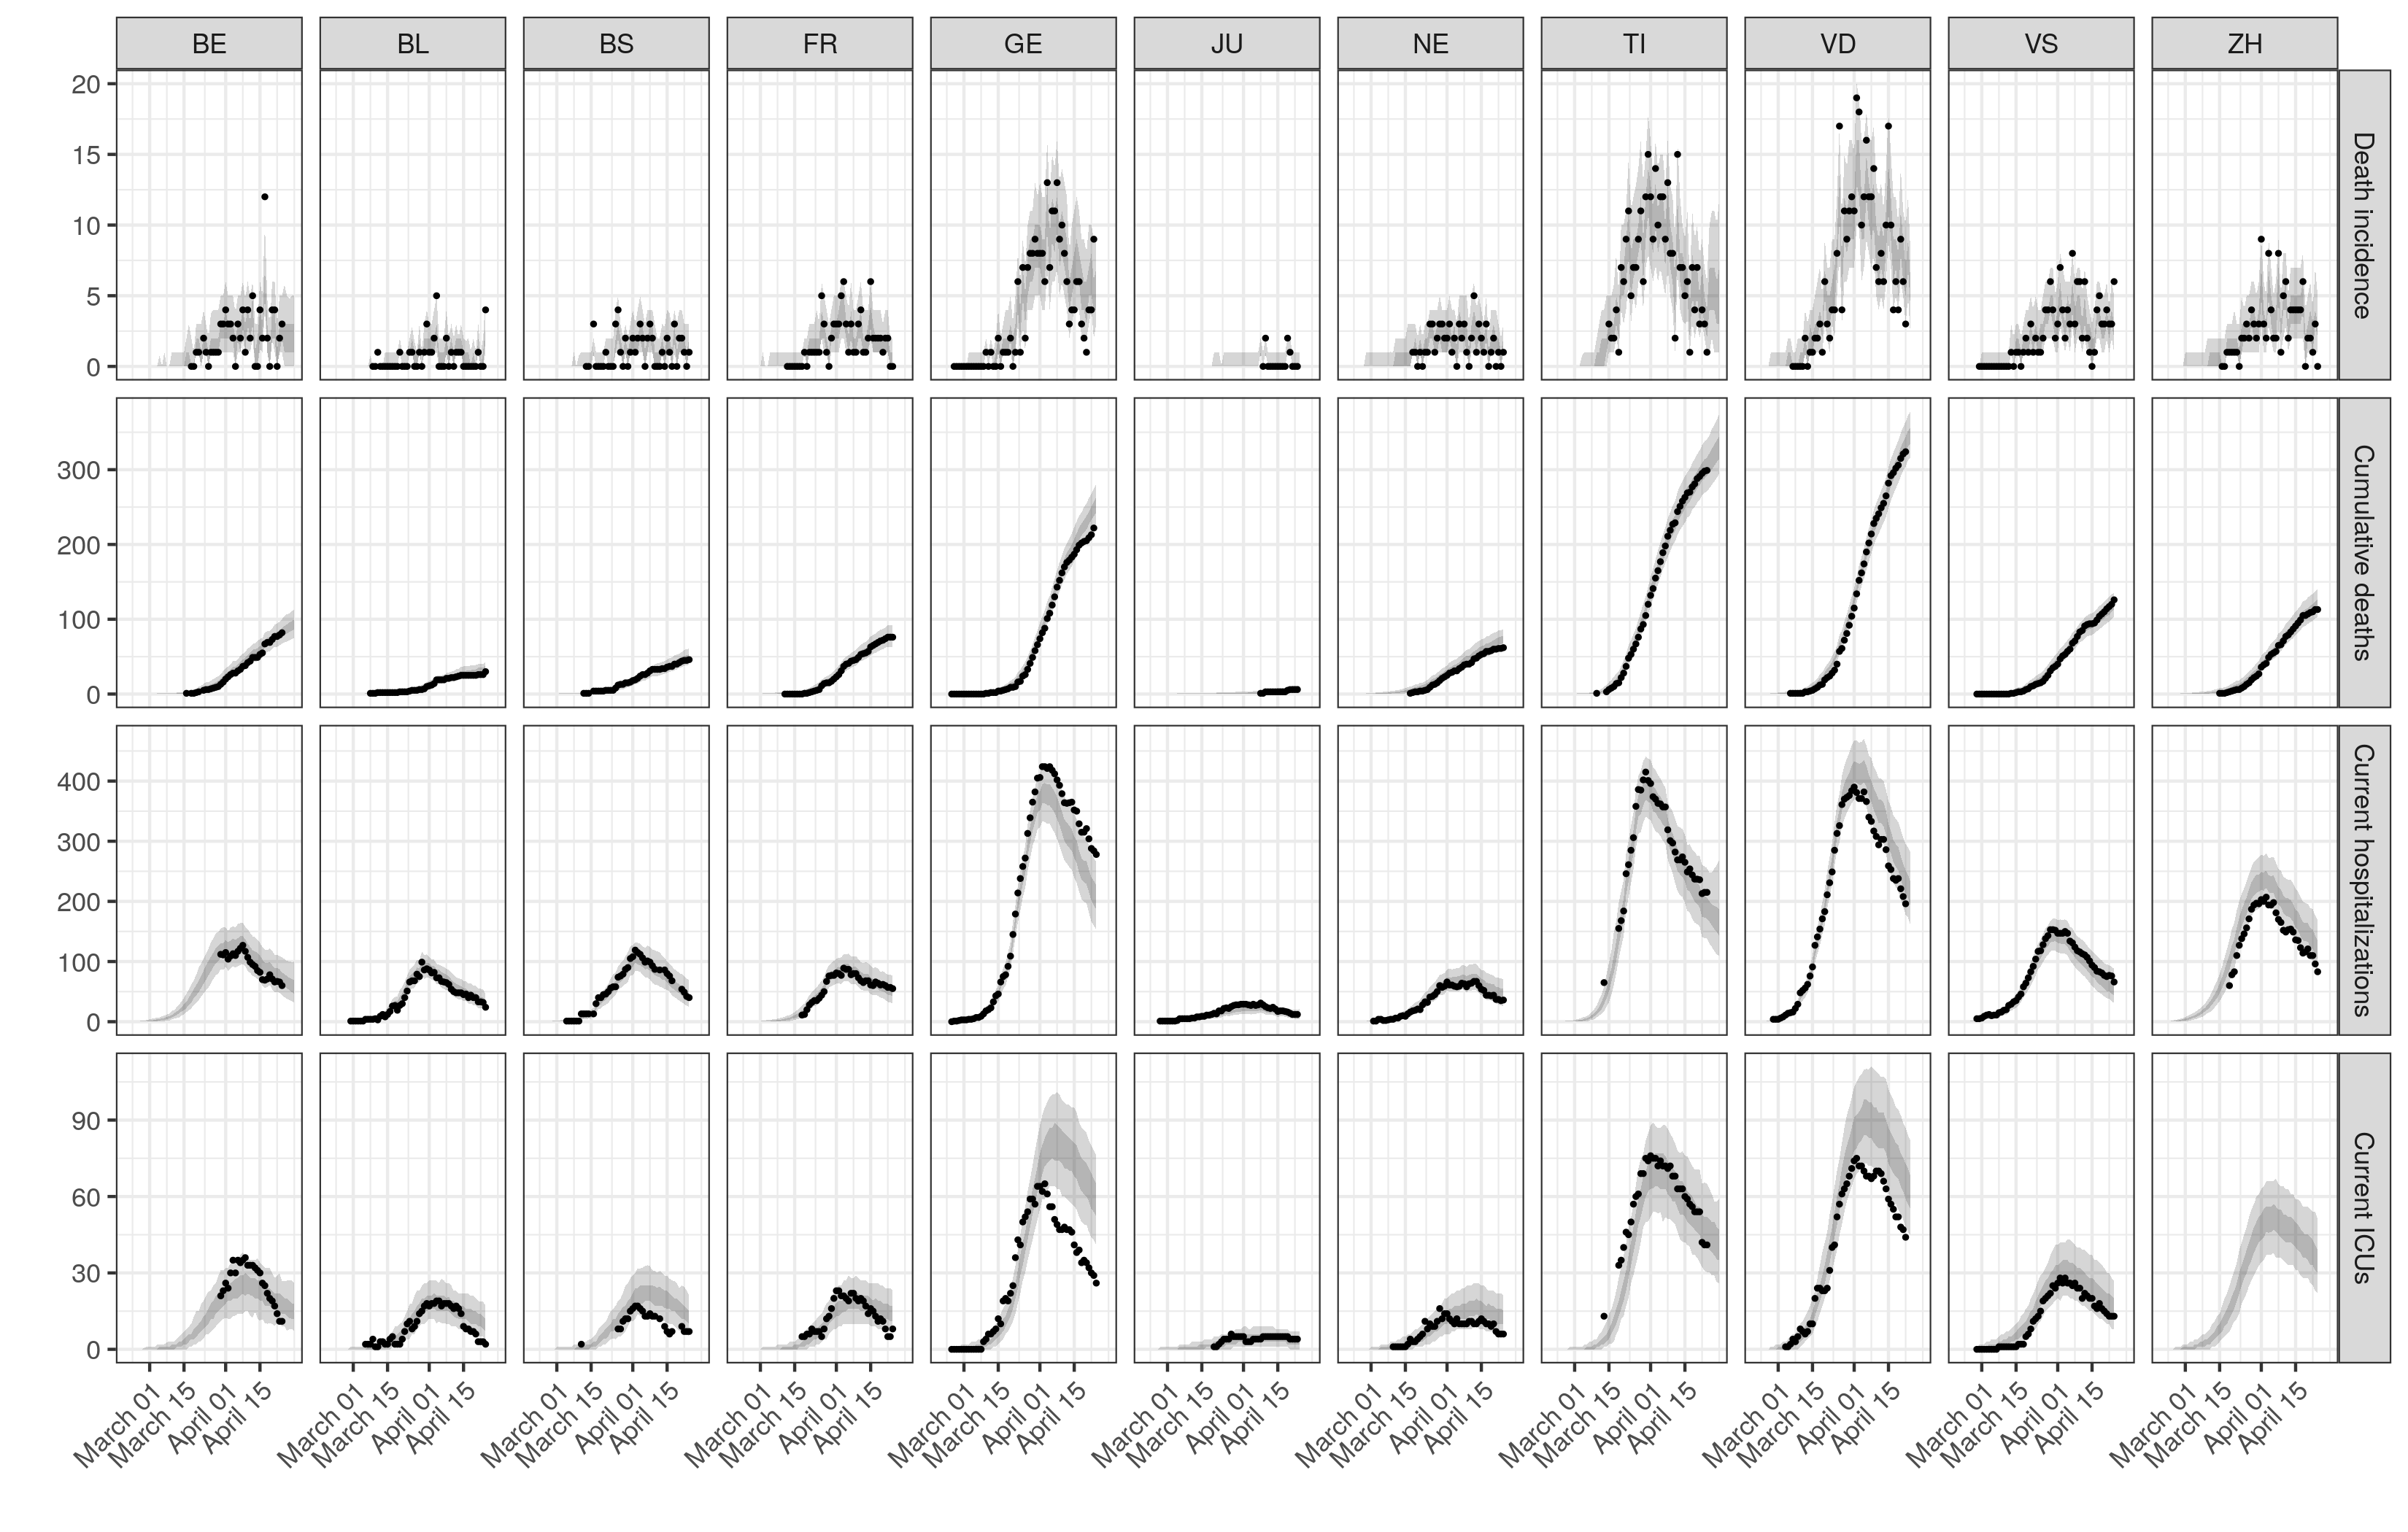
\includegraphics{fig_covid-switzerland-npi/fig_supp/caton_fits.png}
%    \caption[Cantonal level fits]{Cantonal level fits, with the same legend as in fig.~\ref{fig:chfit}. Data (points) from \textcite{openZH:OpenZHCovid19:2020}.}
%    \label{fig:cantonfit}
%\end{figure}



%\begin{figure}
%    \centering
%    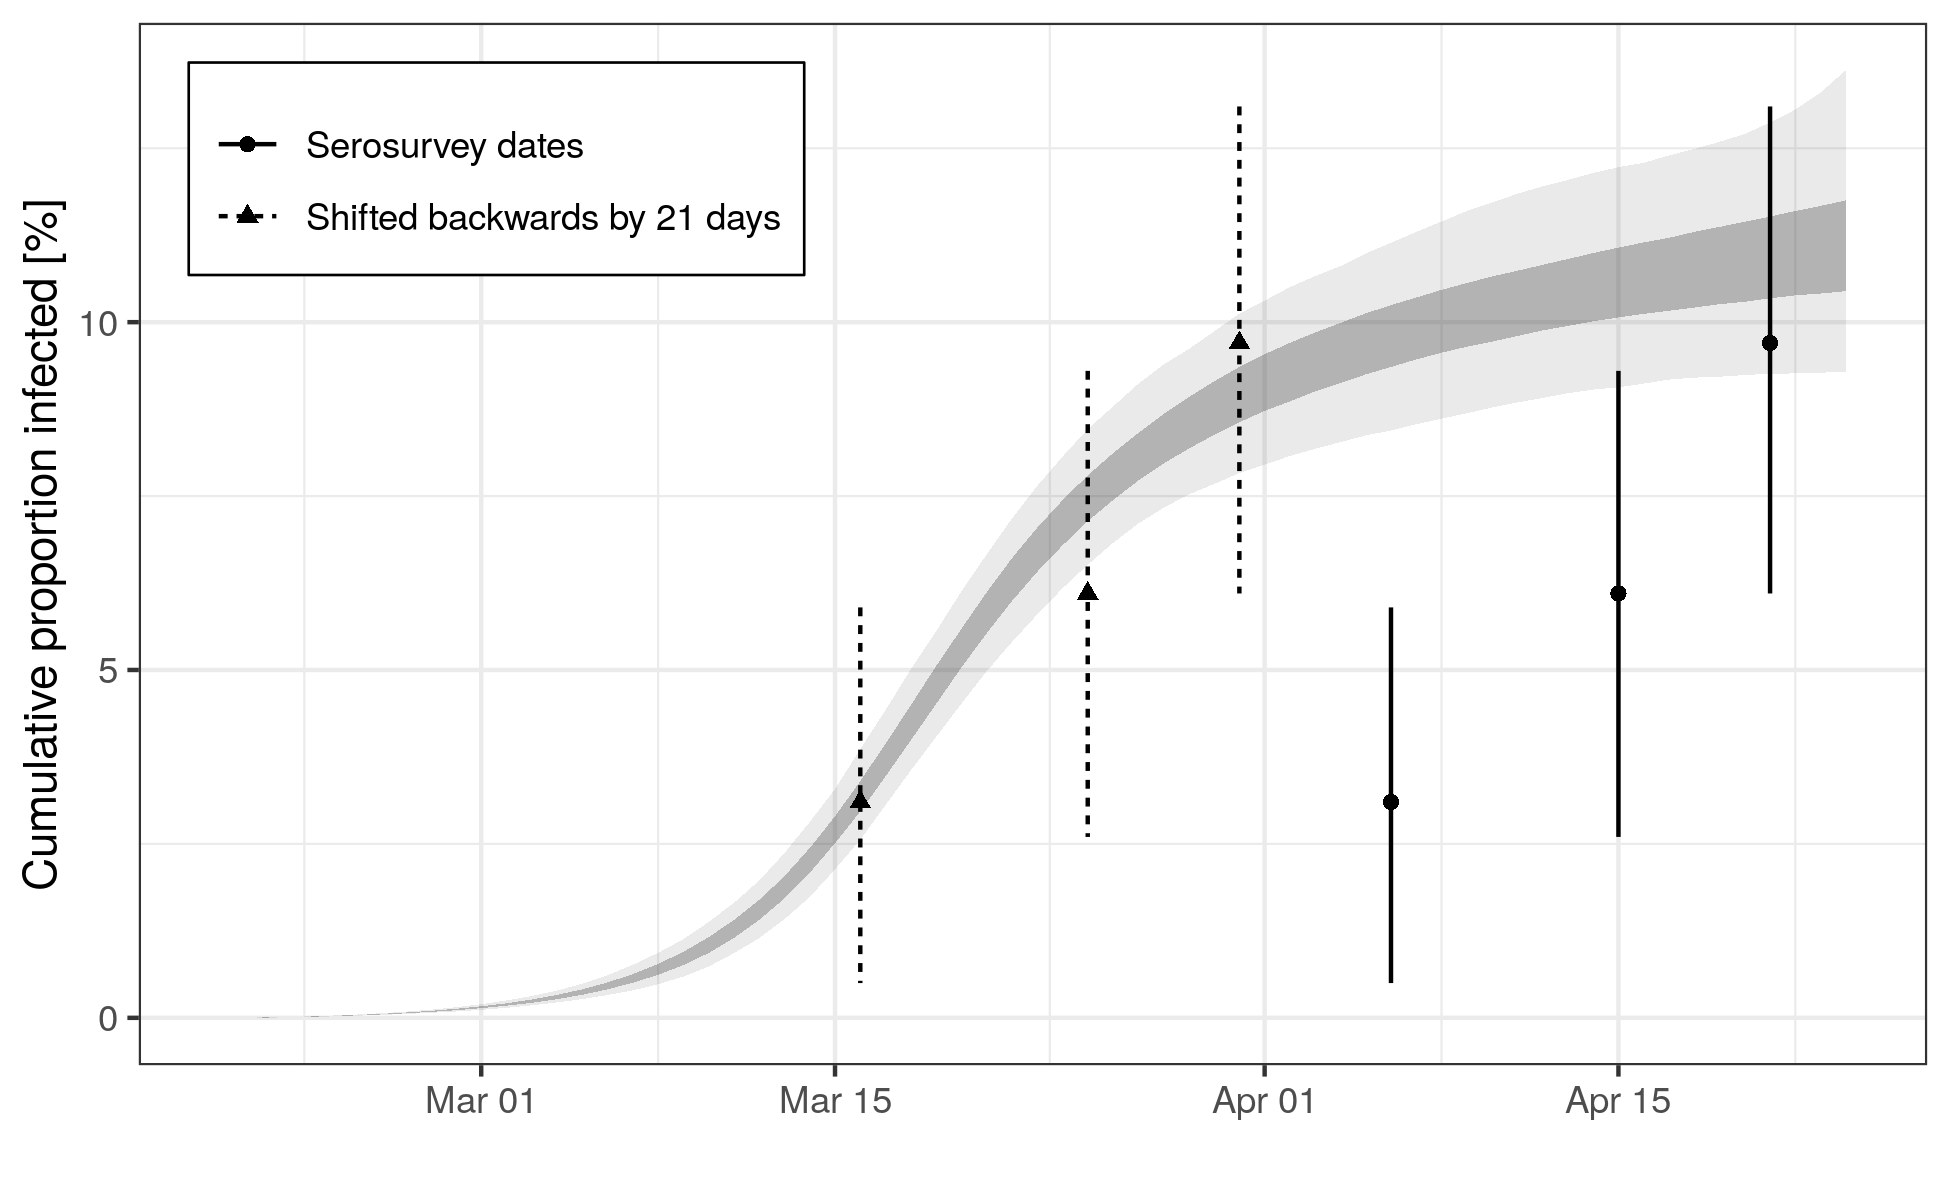
\includegraphics[width=.8\textwidth]{fig_covid-switzerland-npi/fig_supp/GE_seroprevalence_comparison.png}
%    \caption[Qualitative comparison between modelled infected in the canton of Genève and seroprevalence estimates]{Qualitative comparison between modelled proportion of people infected in the canton of Genève and seroprevalence estimates. Model estimates (ribbons, dark shading give the IQR and light shading the 95\% quantile range) are compared to seroprelavence estimates (points, error bars give the 95\% CrI)   taken from Figure 1 in \parencite{stringhini_repeated_2020} [Accessed May 15 2020]. Seroprevalence estimates do not correspond to infection status on the date of the survey due to the delay between infection and seroconversion. We roughly account for this delay by plotting seropervalence estimates shifted backwards in time to represent the delay between infection and symptom onset (6 days \parencite{bi_epidemiology_2020}) and from symptom onset to seroconversion (about 80\% of seroconversions occur within 15 days \parencite{huang_systematic_2020}), resulting in a total shift of 21 days. Note that seroprevelance estimates were not used in model fitting. Quantitative evaluation of adequacy between modelled proportion infected and seroprevalence estimates would require modelling explicitly seroconversion.}
%    \label{fig:seroprev}
%\end{figure}

%\begin{table}[]
%    \centering
%        \caption[Estimated values of R$_0$ at the beginning of the epidemic]{Estimated values of R$_0$ at the beginning of the epidemic (March 1 to March 10) and after the implementation of non-pharmaceutical interventions (March 29 to April 5). Estimates given in terms of the median and 95\% quantile range (in parenthesis).}
%
%\begin{tabular}{ccccc}
%\toprule
%\multicolumn{1}{c}{ } & \multicolumn{2}{c}{March 01-March 10} & \multicolumn{2}{c}{March 29-April 05} \\
%\cmidrule(l{3pt}r{3pt}){2-3} \cmidrule(l{3pt}r{3pt}){4-5}
% & median & 95\% QR & median & 95\% QR\\
%\midrule
%Switzerland & 2.8 & (2.5-3.1) & 0.4 & (0.27-0.6)\\
%Bern & 2.4 & (2-3) & 0.5 & (0.26-0.9)\\
%Basel-Landschaft & 2.8 & (2.2-3.7) & 0.22 & (0.03-0.7)\\
%Basel-Stadt & 3.1 & (2.6-3.8) & 0.3 & (0.13-0.6)\\
%Fribourg & 2.7 & (2.2-3.4) & 0.4 & (0.2-0.8)\\
%Geneve & 2.6 & (2.1-3) & 0.5 & (0.24-0.8)\\
%Jura & 1.4 & (1.2-1.6) & 0.7 & (0.4-1)\\
%Neuchatel & 2 & (1.7-2.3) & 0.6 & (0.4-1)\\
%Ticino & 4 & (3-5) & 0.5 & (0.29-1)\\
%Vaud & 2.7 & (2.4-3) & 0.5 & (0.3-0.8)\\
%Valais & 1.8 & (1.4-2.2) & 0.29 & (0.07-0.7)\\
%Zurich & 2.3 & (1.8-2.8) & 0.5 & (0.25-0.9)\\
%\bottomrule
%\end{tabular}
%    \label{tab:r0}
%\end{table}
%
%
%\begin{table}[]
%    \centering
%     \caption[Estimated proportion of population infected with SARS-CoV-2 as of April 24 2020]{Estimated proportion of population infected with SARS-CoV-2 as of April 24 2020. Estimates given in terms of the median and 95\% quantile range (in parenthesis).}
%\begin{tabular}{ll}
%\toprule
%Canton & Proportion infected [\%]\\
%\midrule
%Switzerland & 3.9 (3.6-4.3)\\
%Bern & 1.9 (1.4- 2.6)\\
%Basel-Landschaft & 3.9 (2.9-5.0)\\
%Basel-Stadt & 6.7 (5.0-8.6)\\
%Fribourg & 4.0 (3.0-5.4)\\
%Geneve & 11.0 (9.3-13.3)\\
%Jura & 4.2 (2.8- 6.5)\\
%Neuchatel & 6.7 (4.9-9.1)\\
%Ticino & 16.0 (13.5-21.2)\\
%Vaud & 8.0 (6.8- 9.3)\\
%Valais & 5.5 (4.4-7.4)\\
%Zurich & 2.3 (1.8- 2.9)\\
%\bottomrule
%\end{tabular}
%    \label{tab:infection}
%\end{table}





\chapter{Appendix to chapter 6}

\section{Comment on the simplifications}
\paragraph{Discussion on Simplification (a).}
Realistically, vaccinations will occur at least eight hours per day. The assumption, while justified as a computationally convenient approximation of reality, is not a priori worse than assuming that vaccine administration takes place over the whole day. More refined approximations, while in principle possible, pose severe issues because of the nature of the system dynamics. While for most initial values the system dynamics can be easily simulated with time-continuous vaccinations, the system becomes stiff by construction once almost the entire population has been vaccinated. In this case, numerical integration errors can drive the size of some compartments to be negative, which violates the model assumptions and makes the result of the numerical integration meaningless. The main issue in this case is that the optimizer will exploit these inaccuracies in order to reduce the cost. Therefore, this issue is much more evident when solving optimal control problems than when simply simulating the system dynamics. Some simple approaches to tackle this issue are investigated, but no technique yielded satisfactory performances. It is our impression that ad-hoc integration strategies will be required in order to reliably simulate and optimize dynamics with continuous vaccination rates. While this will be the subject of future research, the results obtained with the current approximation have yielded sufficient accuracy.

\paragraph{Discussion on Simplification (b).}
This simplification has been proposed in~\cite{Savorgnan:MultipleShootingDistributed:2011} as an approach to solve distributed optimal control problems by means of multiple shooting. In the original version, the coupling variable $z$ is not necessarily piecewise constant, but rather piecewise polynomial. In simulations of this problem, the piecewise constant parametrization has been observed to yield sufficient accuracy.

The dynamics of each node are discretized using an explicit Runge-Kutta integrator of order four, with $50$ integration steps per day. Alternative integrators such as explicit Euler, or implicit Runge-Kutta integrators, yielded similar results. Furthermore, in order to verify the accuracy of the integrator and the impact of the introduced simplifications on the solution accuracy, the system is simulated in open-loop, i.e. the optimal control trajectory is applied to the full model starting from the initial condition provided by the data assimilation scheme.

\paragraph{Discussion on Simplification (c).} The mobility matrix is sparsified by pruning element below a threshold (see fig.~\ref{figSI:mobility_simplification}). This operation reduces the number of connection between nodes. Also in this case, the introduced simplification has been verified through numerical simulations to have a small impact on the prediction and control accuracy.

\begin{figure*}
\centering
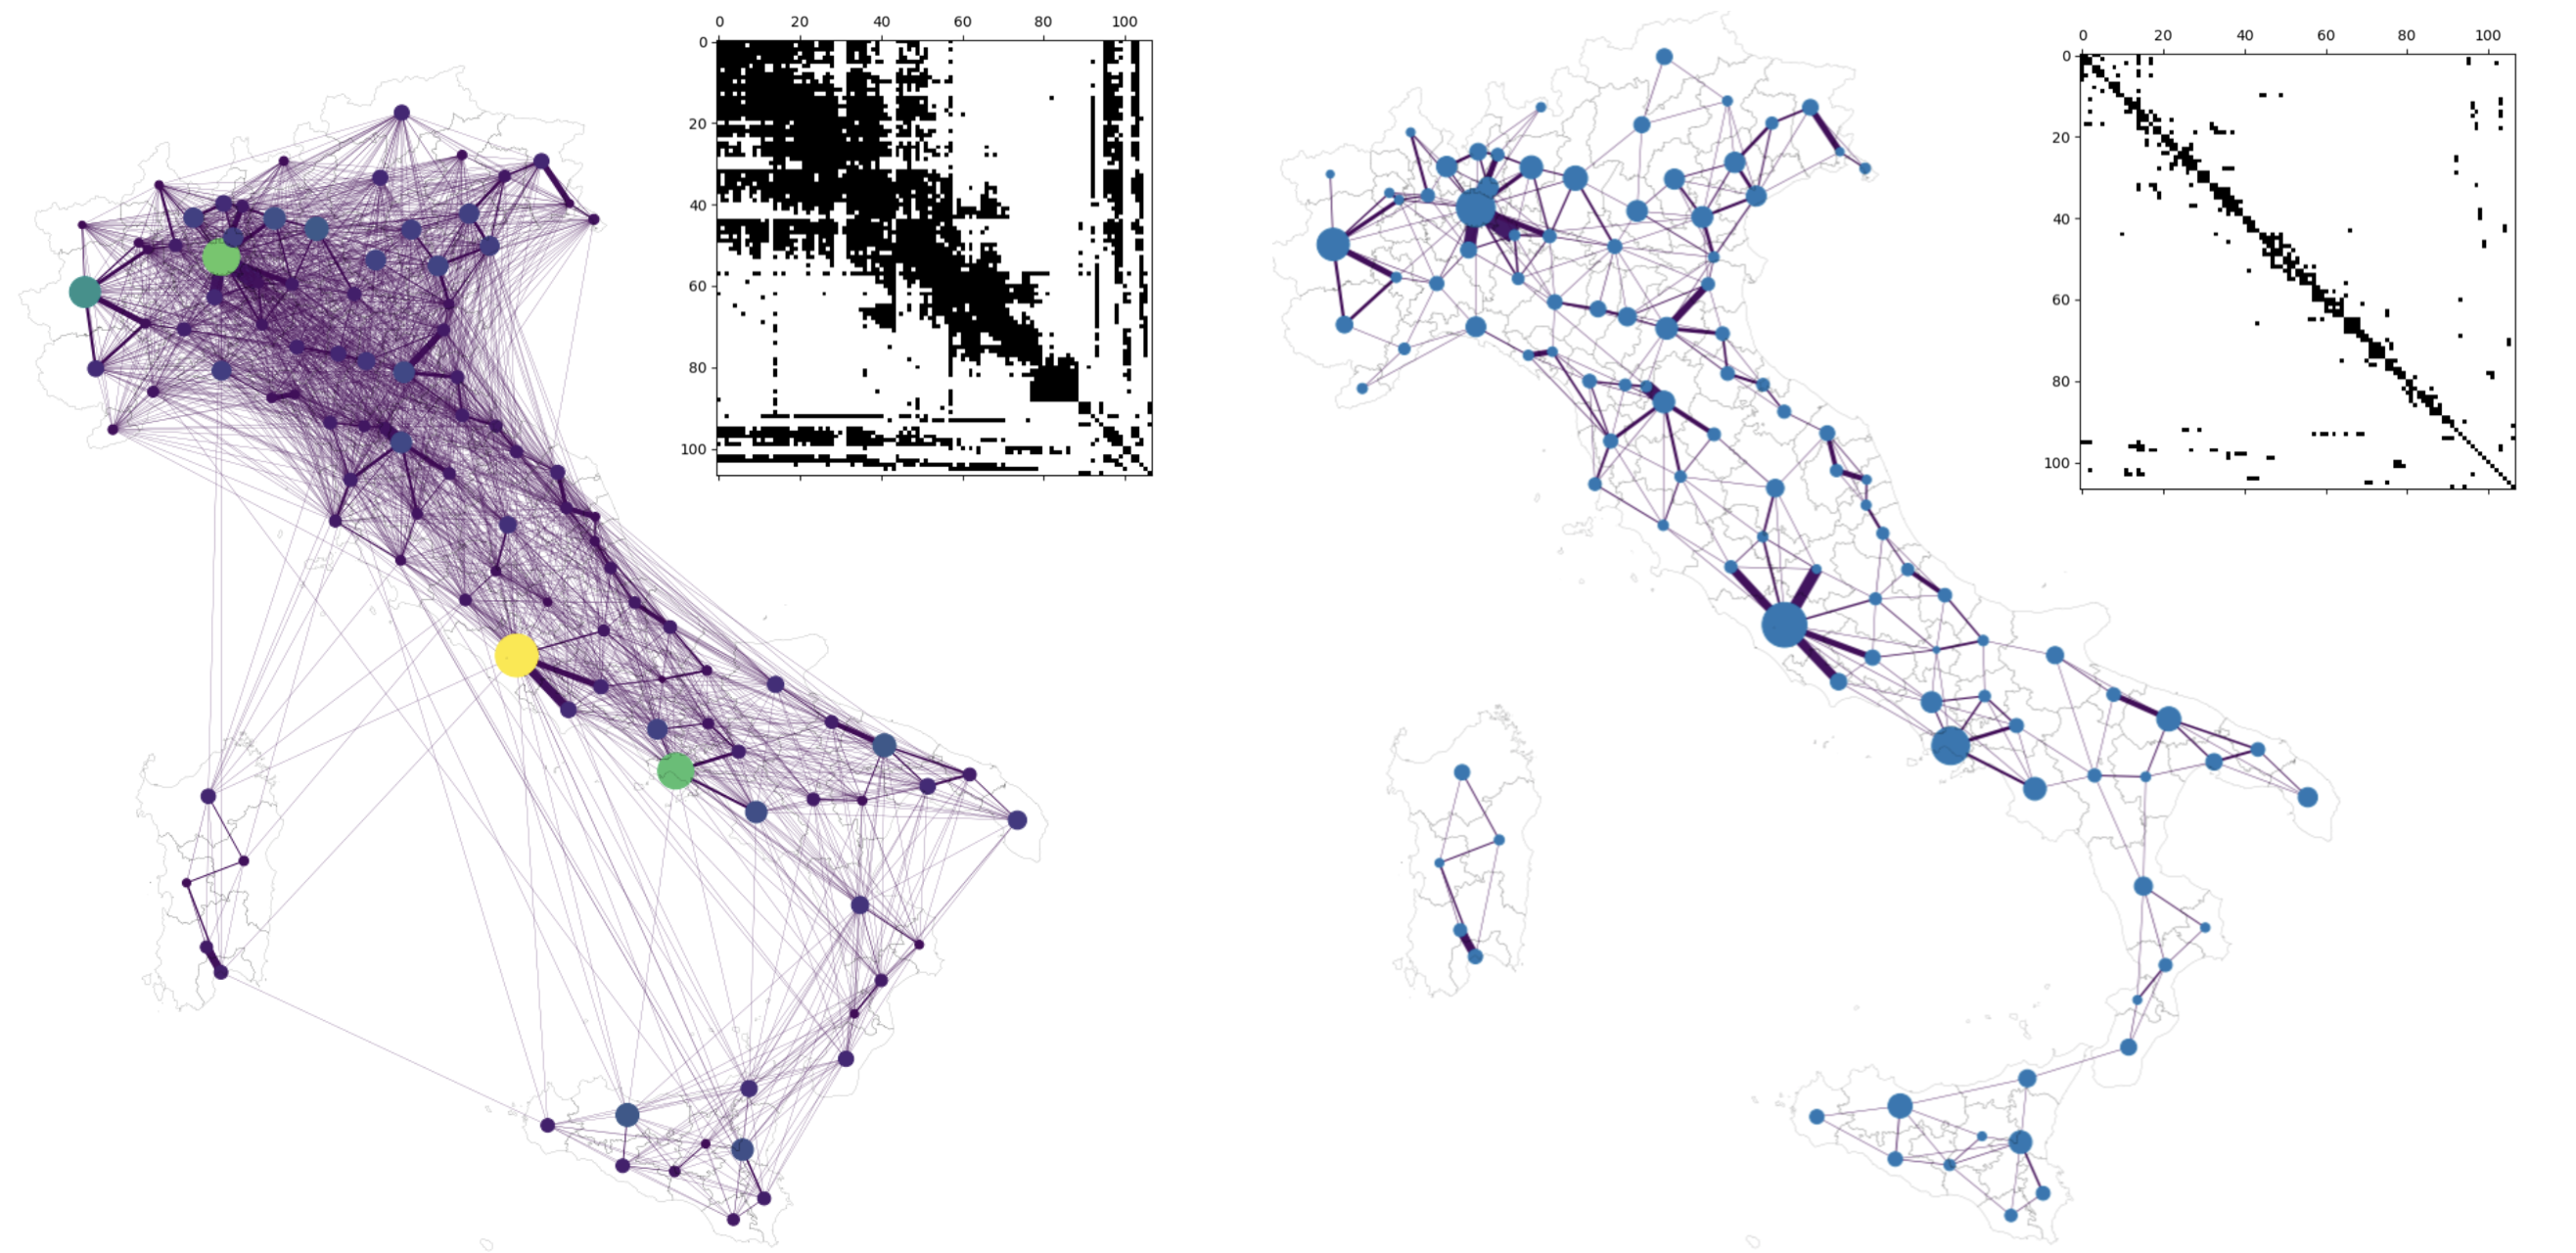
\includegraphics[width=\textwidth]{fig_italy-ocp/figuresSI/mobsimplification.png}
\caption[Simplification of the mobility matrix to obtain a sparse and tractable problem]{Simplification of the mobility matrix to obtain a sparse and tractable problem. After the optimization, the effectiveness of the optimal control strategy is assessed on the full model.} \label{figSI:mobility_simplification}
\end{figure*}

\paragraph{Possible further improvements} Applying optimal control in open loop, i.e., solving the optimization problem once and applying the control input over the whole time interval, may lead to poor performance due to model inaccuracy and external perturbations. A common remedy consists in closing the loop by repeatedly solving the OCP by using the most updated information on the initial states. This is the principle behind Model Predictive Control (MPC)~\cite{Rawlings:ModelPredictiveControl:2017}. In this context, the state would be estimated on a daily, weekly, or monthly basis so as to solve again the OCP and correct the optimal strategy.


%% ***********************************************************************************************
%\section{Data assimilation and model parameters}
%% ***********************************************************************************************
%\begin{figure*}
%    \centering
 %   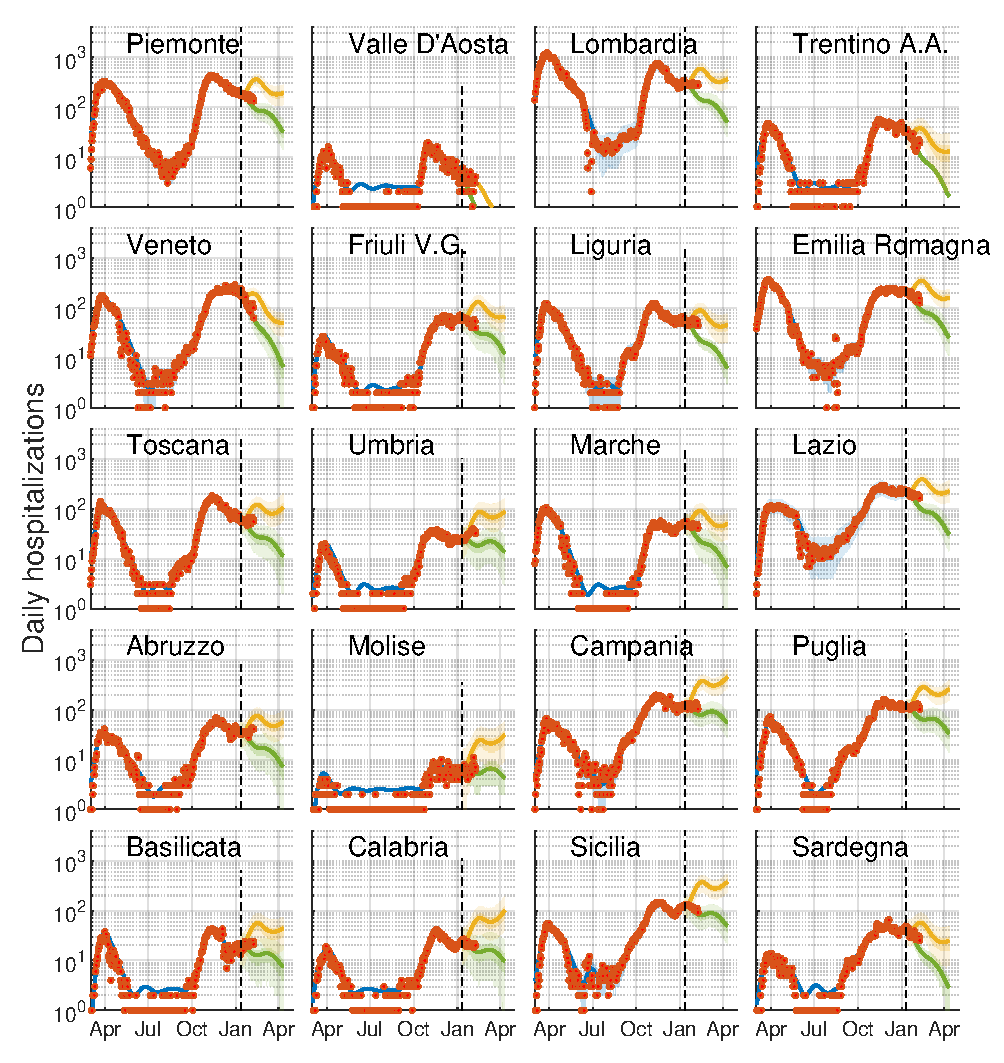
\includegraphics[width=1\textwidth]{fig_italy-ocp/figuresSI/DA_all_sim/hosp.pdf}
  %  \caption[Modeled daily hospitalizations the against hospitalization data]{Modeled daily hospitalizations (blue) versus hospitalization data (red dots), regional detail of fig. 2.A in the main text. The optimistic and pessimistic transmission scenarios are represented in green and yellow, respectively.}
%    \label{fig:SI_DA1}
%\end{figure*}
%\begin{figure*}
%    \centering
%    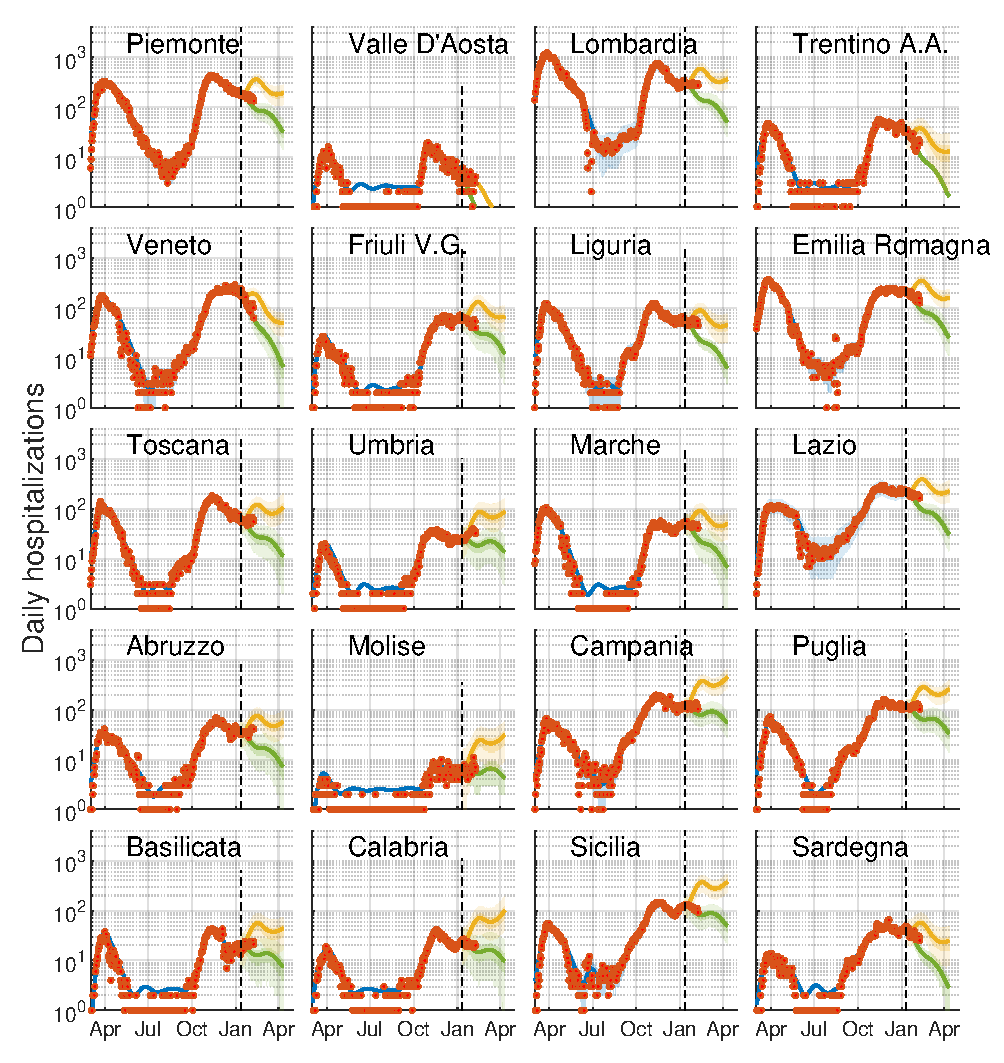
\includegraphics[width=1\textwidth]{fig_italy-ocp/figuresSI/DA_all_sim/incidence.pdf}
%    \caption[Modeled daily incidence against the daily reported cases]{Modeled daily incidence (blue) versus the daily reported cases (red dots), regional detail of fig. 2.B in the main text. The optimistic and pessimistic transmission scenarios are represented in green and yellow, respectively.}
%    \label{fig:SI_DA2}
%\end{figure*}

%The regional transmission rates are the main parameters governing the force of infection of the model and, thus, the daily exposed individuals. To better track possible changes in the transmission rates, w- adopt a data assimilation strategy based on an iterative particle filter\cite{Manoli:IterativeParticleFilter:2015} used on a moving window of 14 days. The filter starts considering $N_r=1000$ model realizations at time $t_0$ (February 21, 2020), whose state variables are $x_0^{(j)}, j=1,\dots, N_r$, where the superscript $(j)$ is the realization index and the subscript is the temporal index. Each realization is associated with a parameter combination that is randomly sampled from the posterior distribution evaluated in\cite{Bertuzzo:GeographyCOVID19Spread:2020}, indicated with $\theta^{(j)}$. Possible spatial heterogeneities in regional transmission on a given day $t_k$ are obtained multiplying the transmission parameter by a coefficient $\phi_{k,i}^{(j)}$, where $i$ is the region's index. At time $t_0$, the coefficients $\phi_{0,i}^{(j)}$ are sampled from a truncated normal distribution (mean $\mu_0=1$, standard deviation 0.4, bounds $0.8\mu$-$1.2\mu_0$).
%At time $t_k$, w- assume to know the state variables $x_k^{(j)}$ and coefficients $\phi_{k,i}^{(j)}$, the latter having ensemble mean $\mu_{k,i}$. To update state variables and coefficients at time $t_{k+1}$, w- consider the observations (daily hospitalizations) collected in a temporal window of $\tau=14$ days, $(t_k,t_{k}+\tau$. New coefficients from the truncated normal distribution (mean $\mu_k=1$, standard deviation 0.4, bounds $0.8\mu_k$-$1.2\mu_k$) are sampled at time $\tau=t_0+14$ days.  For each realization, w- run the model during the window of 14 days, assuming that the coefficients change linearly for a week, from  $\phi_{0,i}^{(j)}$ to $\tilde{\phi}_{0,i}^{(j)}$, and remain constant afterwards.
%The regional likelihood of each realization is then evaluated during these two weeks considering that the daily hospitalizations follow a gamma distribution (as in\cite{Bertuzzo:GeographyCOVID19Spread:2020}). 
%A resampling step (systematic resampling , see, e.g.\cite{Douc:ComparisonResamplingSchemes:2005}) selects and duplicates the coefficients $\tilde{\phi}_{0,i}^{(j)}$ associated with the largest likelihood values. These coefficients are then used to update the mean value $\mu_k$. Finally, the simulation is repeated on the same temporal window by sampling new coefficients $\tilde{\phi}_{0,i}^{(j)}$ from the truncated normal distribution with the updated mean $\mu_k$. This set of coefficients is used to compute state variables and parameters at time $t_k$, and then as starting condition to produce the projections used in the main text.

%Model parameters (in the absence of vaccination) are taken from a paper\cite{Bertuzzo:GeographyCOVID19Spread:2020} where they were inferred in a Bayesian framework for the period February~24 -- May~1, 2020, on the basis of the official epidemiological bulletins released daily by Dipartimento della Protezione Civile\cite{DipartimentodellaProtezioneCivile:EmergenzaCoronavirusRisposta} (data available online at {\url{https://github.com/pcm-dpc/COVID-19}}) and the bulletins of Epicentro, at Istituto Superiore di Sanit{à}\cite{IstitutoSuperiorediSanita:CoronavirusUltimiAggiornamenti:2020,Palmieri:CharacteristicsCOVID19Patients:2020}. All the parameters estimated for the initial phase of the Italian \textsc{covid}-19 epidemic, including the transmission rates, are spatially homogeneous\cite{Bertuzzo:GeographyCOVID19Spread:2020}. This parameterization has been used to produce all the results presented in the main text.


%% ***********************************************************************************************
\paragraph{Spatial set-up} 
%% ***********************************************************************************************
The modeling tools described in the following sections are applied to the Italian \textsc{covid}-19 epidemic at the scale of second-level administrative divisions, i.e. provinces and metropolitan cities (currently, as of 2021, $107$ spatial units). Official data about resident population at the provincial level is produced yearly by the Italian National Institute of Statistics (Istituto Nazionale di Statistica, ISTAT; data available at\\ \url{http://dati.istat.it/Index.aspx?QueryId=18460}). The latest update (January 1, 2019) has been used to inform the spatial distribution of the population. %For the age-stratified model the data also comes from ISTAT, in the 2018 census: \url{http://demo.istat.it/popres/index.php?anno=2018&lingua=eng}.
The data to quantify nation-wide human mobility come from ISTAT (specifically, from the 2011 national census; data available online at \url{https://www.istat.it/it/archivio/139381}). Mobility fluxes, mostly reflecting commuting patterns related to work and study purposes, are provided at the scale of third-level administrative units (municipalities)\cite{Pepe:COVID19OutbreakResponse:2020,Vollmer:Report20Using:2020}. These fluxes were upscaled to the provincial level following the administrative divisions of 2019, and used to evaluate the fraction $p_i$ of mobile people in each node~$i$, as well as the fraction $q_{ij}$ of mobile people who move between~$i$ and all other administrative units~$j$ (see Supplementary Material in\cite{Gatto:SpreadDynamicsCOVID19:2020}).
The epidemiological data is obtained from the bulletins of the Dipartimento della Protezione Civile, \url{https://github.com/pcm-dpc/COVID-19}).

%% ***********************************************************************************************
\section{Details of the alternative strategies}
%% ***********************************************************************************************
Alternative strategies are created to be compared the optimal solutions. Each strategy uses a decision variable, $\mathcal{V}_i$, as a basis for the allocation of vaccines among provinces. The decision variable is one of:
\begin{itemize}
    \item \textsc{modelled future incidence, absolute}: the modelled total future incidence in a no-vaccination scenario. This is equivalent to the objective of the optimal control problem with no control;
    \item \textsc{modelled future incidence, per population}: as above, but normalized by the resident population in each node;
    \item \textsc{modelled initial susceptibility, absolute}: the modelled number of susceptibles in each province at the start of the vaccination campaign;
    \item \textsc{modelled initial susceptibility, per population}: as above, but normalized by the resident population in each node;
    \item \textsc{province's population}.
\end{itemize}

Two strategies to distribute the doses are defined:
\begin{itemize}
\item \textsc{Focused} Where every province is sorted (higher on top) according to its decision variable $\mathcal{V}_i$. The maximum local rate $v_i^{max}$ is allocated to every province going down through the list, until the stockpile is empty. In other words, assuming an amount $K$ of vaccines is available in the stockpile, the province index $i$ that satisfy $\max_i \mathcal{V}_i$ is searched for, and province $i$ is assigned $M_i = \min(v_i^{max}, K)$ vaccines. Then, the next province $j$ that satisfy $\max_{j,j\neq i} \mathcal{V}_j$ is searched for and assigned $M_j = \min(v_j^{max}, K-M_i)$. And so on, until no vaccine remains in the stockpile. This strategy will concentrate the allocation on nodes with the highest values of the considered decision variable.
\item \textsc{Proportional} In this case, assuming that on a given day there is a quantity of vaccine $K$ in the stockpile, each province $i$ receives an amount $M_i = \min(v_i^{max}, K \cdot \frac{\mathcal{V}_i}{\sum_j \mathcal{V}_j})$. This approach vaccinate each node proportionally to the value of its decision variable $\mathcal{V}_i$.
\end{itemize}
In the main text, the results for three alternative strategies are shown, namely \textit{proportional absolute incidence}, \textit{proportional population}, and \textit{proportional susceptibility}---named respectively Incidence, Population, and Susceptibility. These strategy are good performers across scenarios, and show how different choices for the decision variables may affect the outcomes of the OCP. In the next sections, the results for all these alternative strategies are shown.

%% ***********************************************************************************************
\section{Additional results}
%% ***********************************************************************************************
The results for all these strategies is presented in tab.~\ref{table:all_strat}, and are shown side-by-side in fig.~\ref{fig:OC_comparison_all}. The optimal solutions outperforms all the others solution. In fact, for every given posterior realisation, the optimal control solution always outperforms all other allocation strategies. Even if some scatter is observed when sampling the posterior, the performances of optimal strategies are clearly separated from the rest of the alternatives.

A linear scatter plot of the optimal proportion of vaccinated individuals per province (sorting variable) side by side with the province population, the projected incidence without vaccination, and the proportion of susceptible individuals at the start of the simulation is presented ro further investigate the features of the optimal solution. These results are presented for the optimistic scenario in fig.~\ref{fig:OC_scatter_optimistic} and for the pessimistic scenario in fig.~\ref{fig:OC_scatter_pessimistic}. No clear visual pattern associating these covariates to the optimal proportion vaccinated is found, highlighting again that the optimal allocation uses the epidemiological variable in a non-straightforward way, different from every simple strategy designed for this exercice.

\begin{fwtable}
\centering
\small
\begin{tabular}{llrrrr}
\toprule
& {} & \multicolumn{2}{c}{Averted Infections} & \multicolumn{2}{c}{Averted Infections} \\
&    &  & & \multicolumn{2}{c}{per dose} \\
Scenario & Method &  Optimistic & Pessimistic &     Optimistic & Pessimistic          \\
\midrule
2M & Optimal &   6.98M &    30.6M &          0.268 &        1.18 \\
        & Incidence &   6.32M &    28.1M &          0.243 &        1.08 \\
        & Proportional Incidence &   6.23M &    27.5M &          0.239 &        1.06 \\
        & Focused Susceptibility &   6.03M &    26.9M &          0.232 &        1.03 \\
        & Focused Proportional Susceptibility &   6.03M &    26.9M &          0.232 &        1.03 \\
        & Focused Proportional Incidence &   6.03M &    26.9M &          0.232 &        1.03 \\
        & Focused Population &   6.03M &    26.9M &          0.232 &        1.03 \\
        & Focused Incidence &   6.03M &    26.9M &          0.232 &        1.03 \\
        & Population &   6.02M &    26.8M &          0.231 &        1.03 \\
        & Susceptibility &   5.97M &    26.7M &          0.229 &        1.02 \\
        & Proportional Susceptibility &    5.6M &    25.3M &          0.215 &       0.971 \\
1.5M & Optimal &   5.52M &    24.1M &          0.283 &        1.24 \\
        & Incidence &   4.89M &    21.7M &           0.25 &        1.11 \\
        & Proportional Incidence &   4.82M &    21.3M &          0.246 &        1.09 \\
        & Focused Population &   4.58M &    20.5M &          0.235 &        1.05 \\
        & Focused Incidence &   4.58M &    20.5M &          0.235 &        1.05 \\
        & Focused Proportional Incidence &   4.58M &    20.5M &          0.235 &        1.05 \\
        & Focused Proportional Susceptibility &   4.58M &    20.5M &          0.235 &        1.05 \\
        & Focused Susceptibility &   4.58M &    20.5M &          0.235 &        1.05 \\
        & Population &   4.57M &    20.4M &          0.234 &        1.05 \\
        & Susceptibility &   4.51M &    20.3M &          0.231 &        1.04 \\
        & Proportional Susceptibility &   4.18M &     19.0M &          0.214 &       0.975 \\
1M & Optimal &    3.9M &    16.9M &            0.3 &         1.3 \\
        & Incidence &   3.41M &    15.1M &          0.262 &        1.16 \\
        & Proportional Incidence &   3.34M &    14.7M &          0.257 &        1.13 \\
        & Focused Population &   3.09M &    13.9M &          0.238 &        1.07 \\
        & Focused Susceptibility &   3.09M &    13.9M &          0.238 &        1.07 \\
        & Focused Proportional Susceptibility &   3.09M &    13.9M &          0.238 &        1.07 \\
        & Focused Incidence &   3.09M &    13.9M &          0.238 &        1.07 \\
        & Focused Proportional Incidence &   3.09M &    13.9M &          0.238 &        1.07 \\
        & Population &   3.08M &    13.8M &          0.237 &        1.06 \\
        & Susceptibility &   3.02M &    13.7M &          0.232 &        1.05 \\
        & Proportional Susceptibility &   2.75M &    12.6M &          0.211 &       0.972 \\
479'700 & Optimal &   1.96M &    8.39M &          0.314 &        1.34 \\
        & Focused Proportional Incidence &   1.95M &    7.74M &          0.312 &        1.24 \\
        & Proportional Incidence &   1.69M &    7.32M &          0.271 &        1.17 \\
        & Incidence &   1.63M &    7.21M &          0.262 &        1.15 \\
        & Focused Incidence &   1.59M &    6.64M &          0.254 &        1.06 \\
        & Focused Population &   1.57M &    6.85M &          0.251 &        1.09 \\
        & Population &   1.45M &    6.57M &          0.233 &        1.05 \\
        & Focused Susceptibility &   1.45M &    6.53M &          0.232 &        1.04 \\
        & Susceptibility &   1.41M &    6.43M &          0.225 &        1.03 \\
        & Focused Proportional Susceptibility &   1.28M &    6.09M &          0.204 &       0.973 \\
        & Proportional Susceptibility &   1.26M &    5.89M &          0.202 &       0.944 \\
\bottomrule
\end{tabular}
\caption{Absolute number of averted infections for each scenario}
\label{table:all_strat}
\end{fwtable}

\begin{fwfigure}
    \centering
    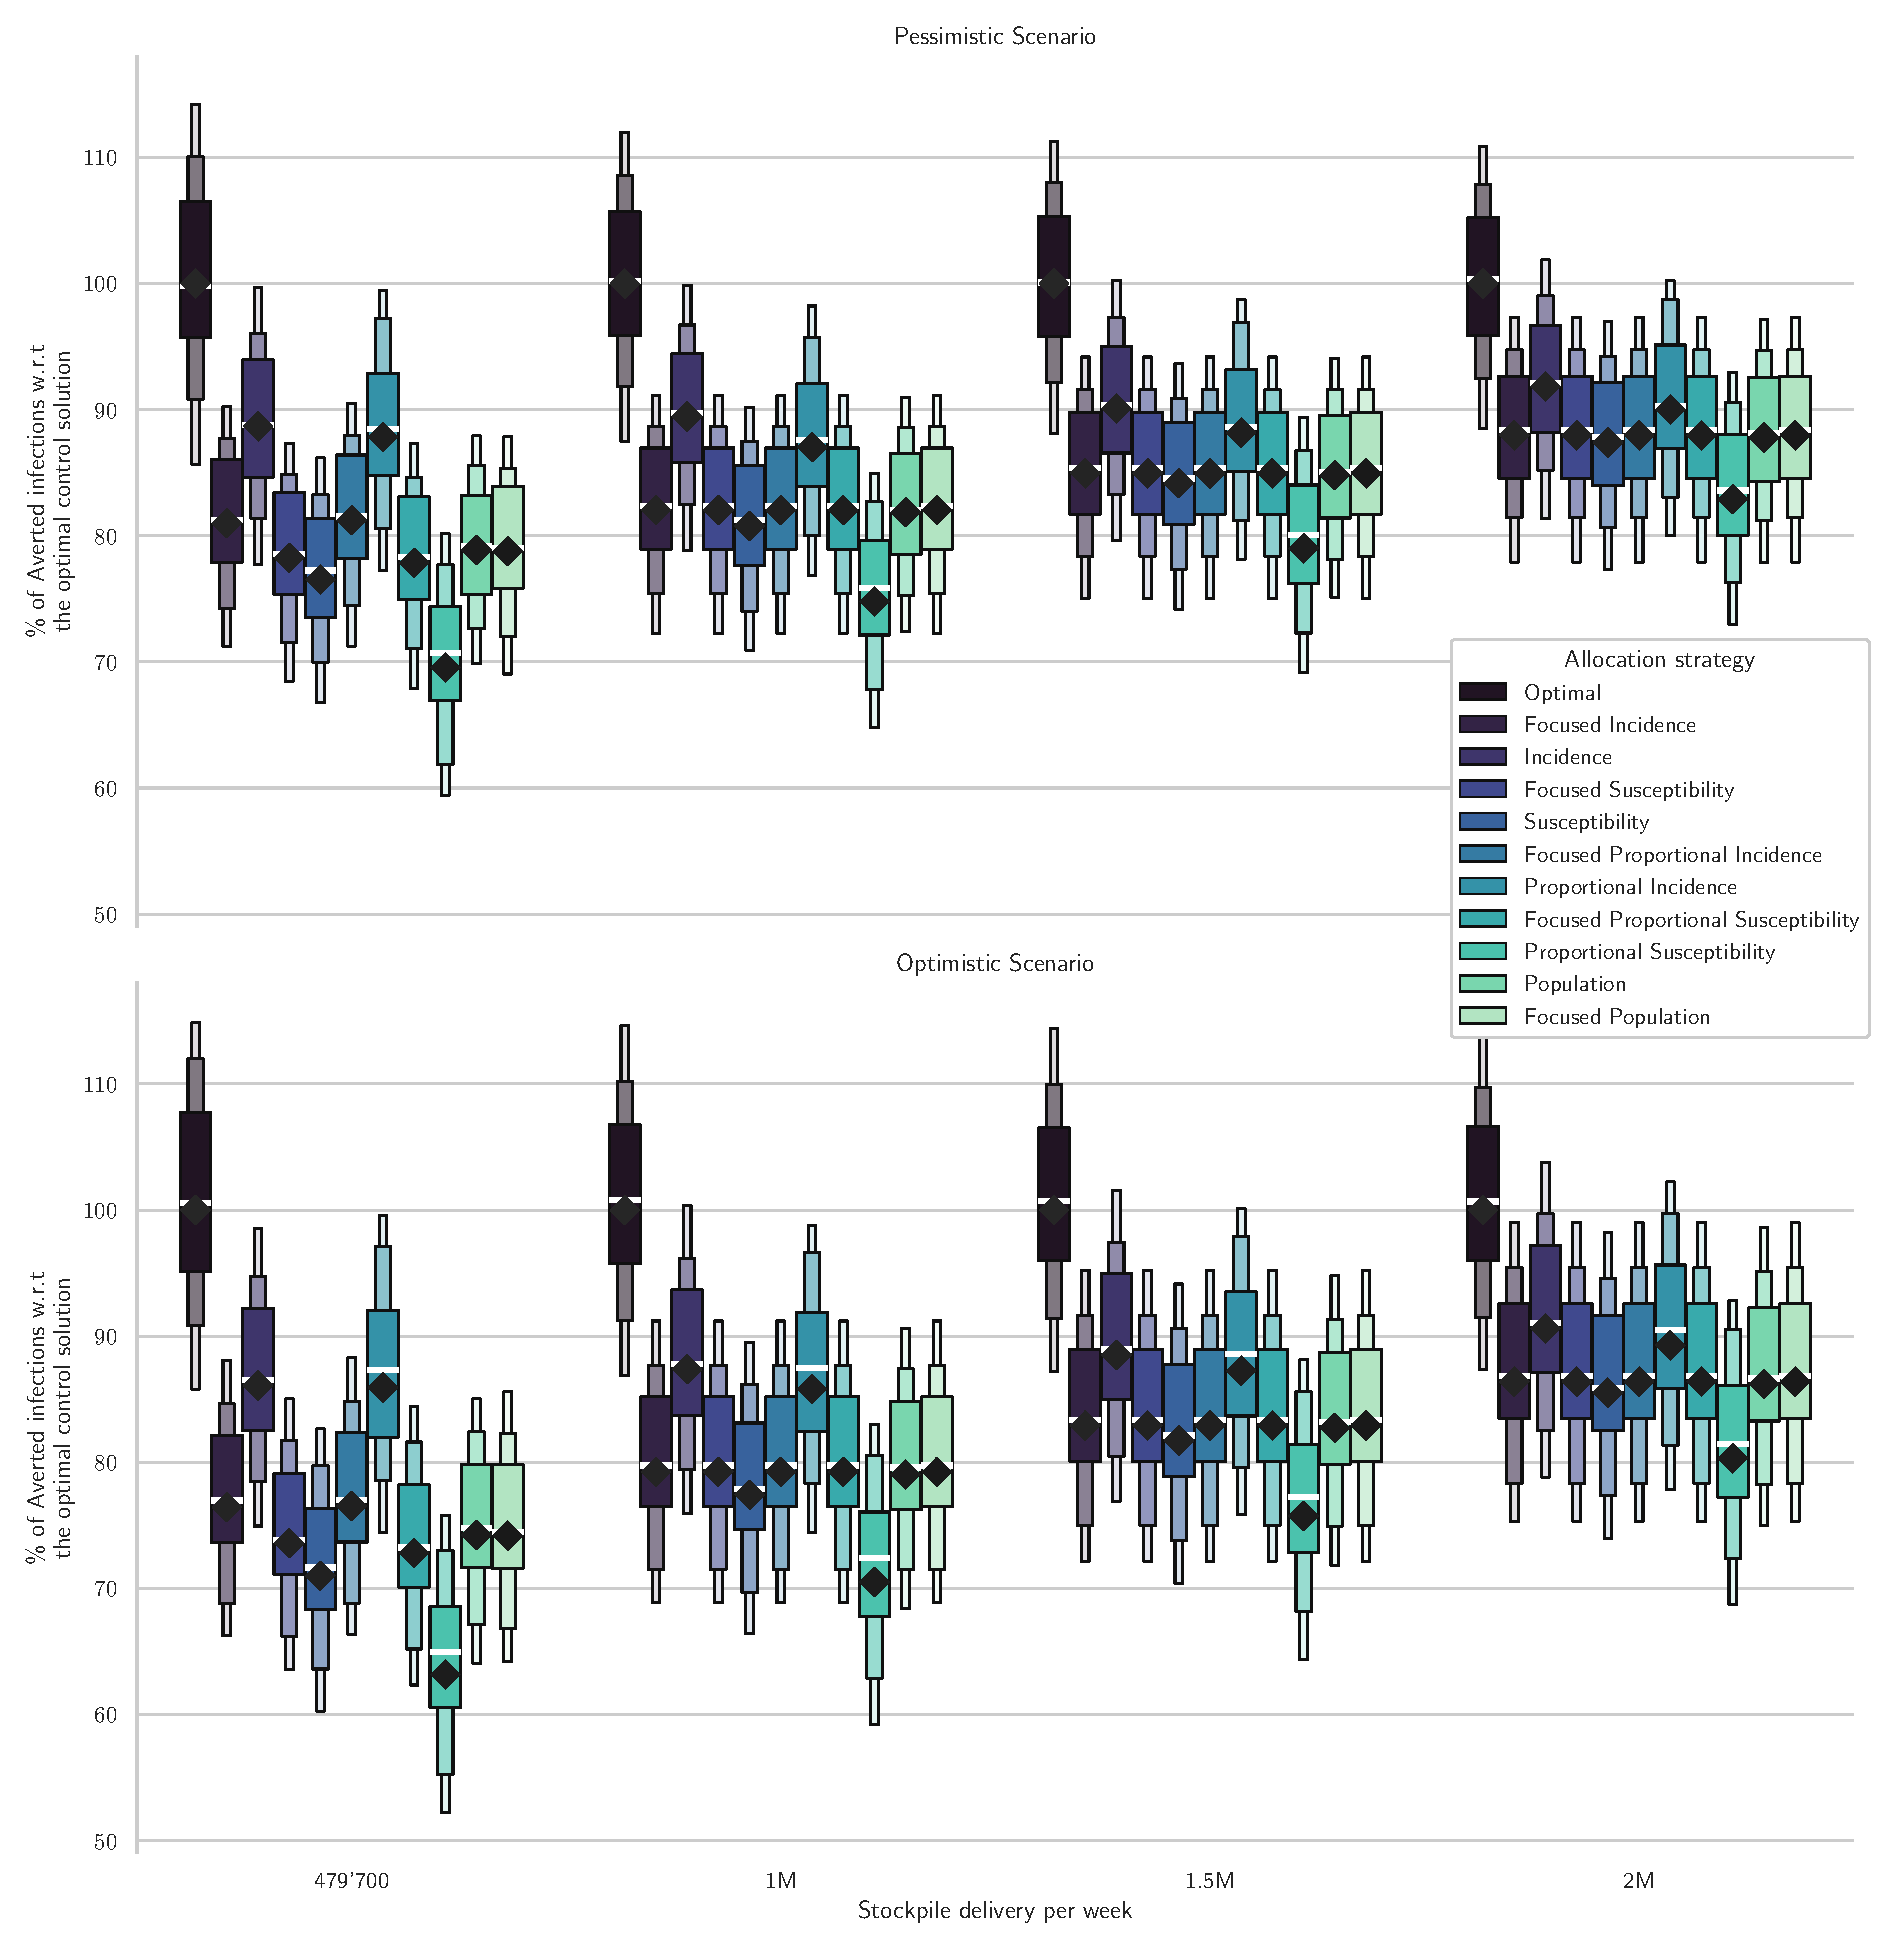
\includegraphics[width=0.9\textwidth]{fig_italy-ocp/figuresSI/scenarios_perturb_all_SI.pdf}
    \caption[Comparison of different allocation strategies]{Comparison of different allocation strategies. Percentages of averted infections per vaccine dose from January 11, 2021 to April 11, 2021 using different vaccine distribution strategies for the pessimistic (panel A) and the optimistic (panel B) scenario based on: the optimal solution, the spatial distribution of the population, the amount of susceptible individuals at the beginning of the vaccination campaign, and the projected disease incidence in the absence of control. A median realization of the modeled posterior is optimized (diamonds), and the performance is assesed on the whole posterior (box plots). The results are normalized by the number of averted infections in the optimized solution (see tab.~\ref{table:all_strat} for absolute values).}
    \label{fig:OC_comparison_all}
\end{fwfigure}


\begin{figure}[!ht]
    \centering
    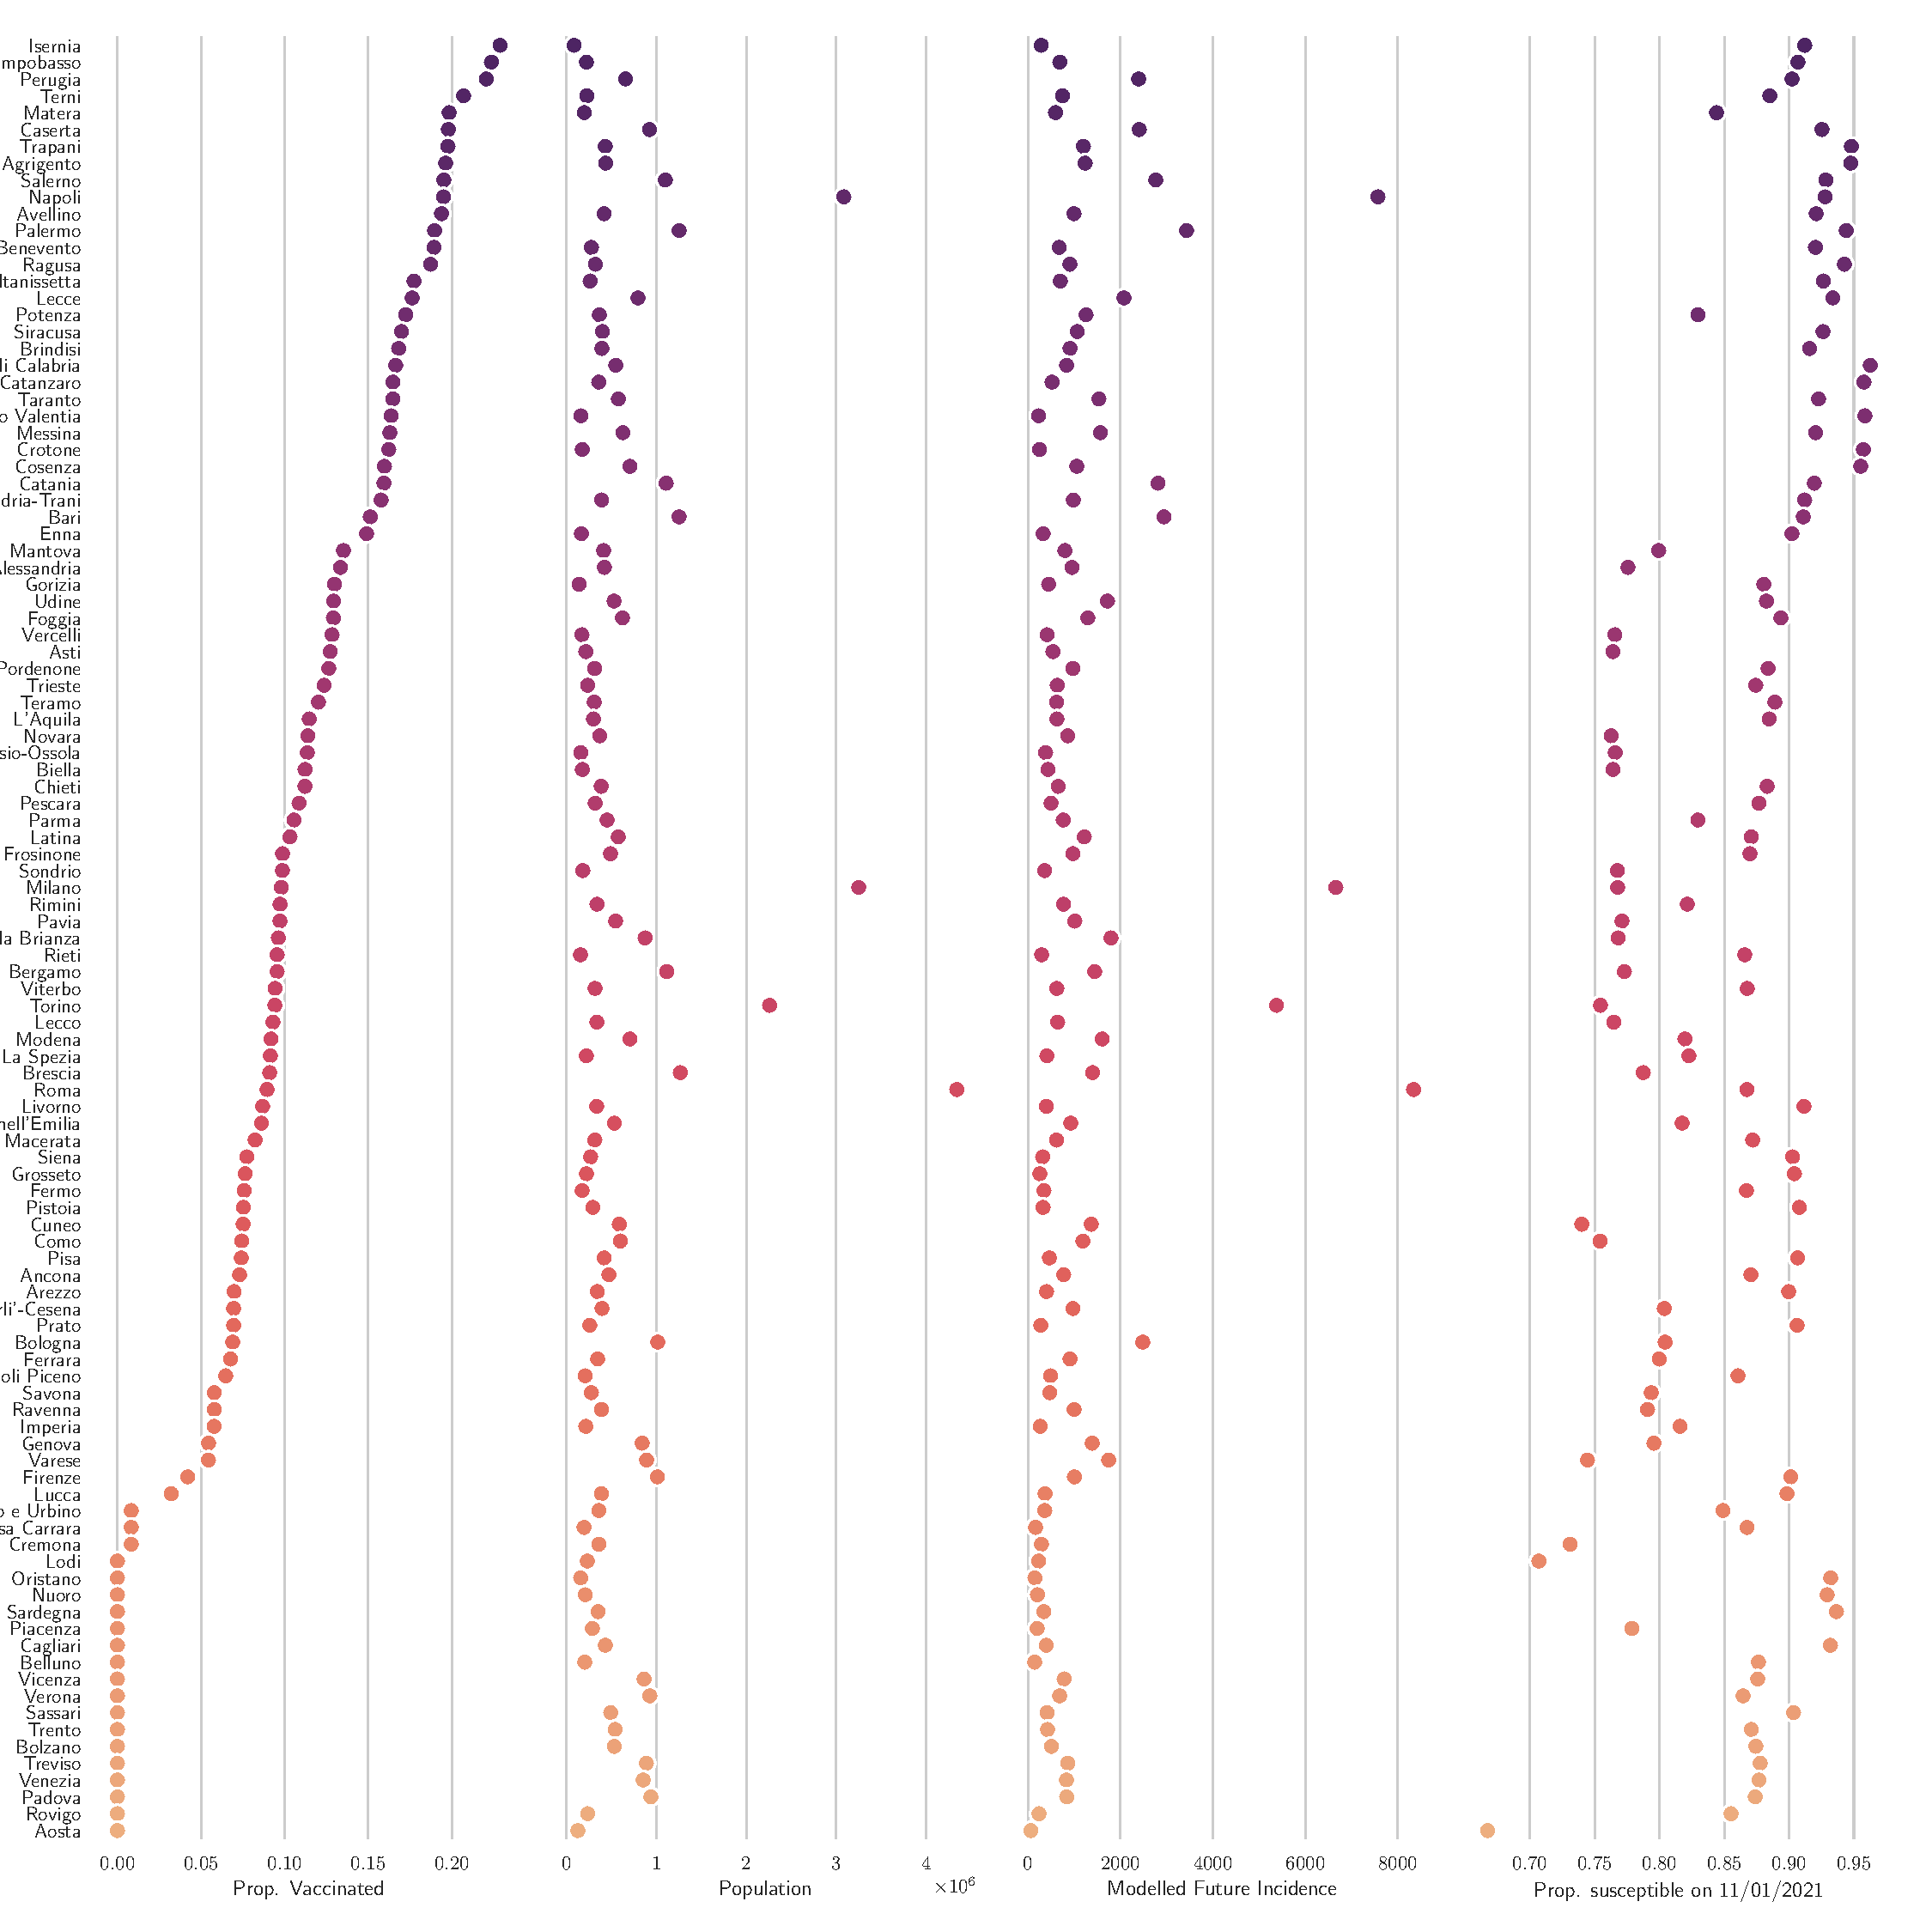
\includegraphics[width=\textwidth]{fig_italy-ocp/figuresSI/SI_scatter_Optimistic.pdf}
    \caption[Control and co-variates for the optimistic scenario]{Control and co-variates for the optimistic scenario with a stockpile delivery of 479'700 vaccine doses.}
    \label{fig:OC_scatter_optimistic}
\end{figure}

\begin{figure}[!ht]
    \centering
    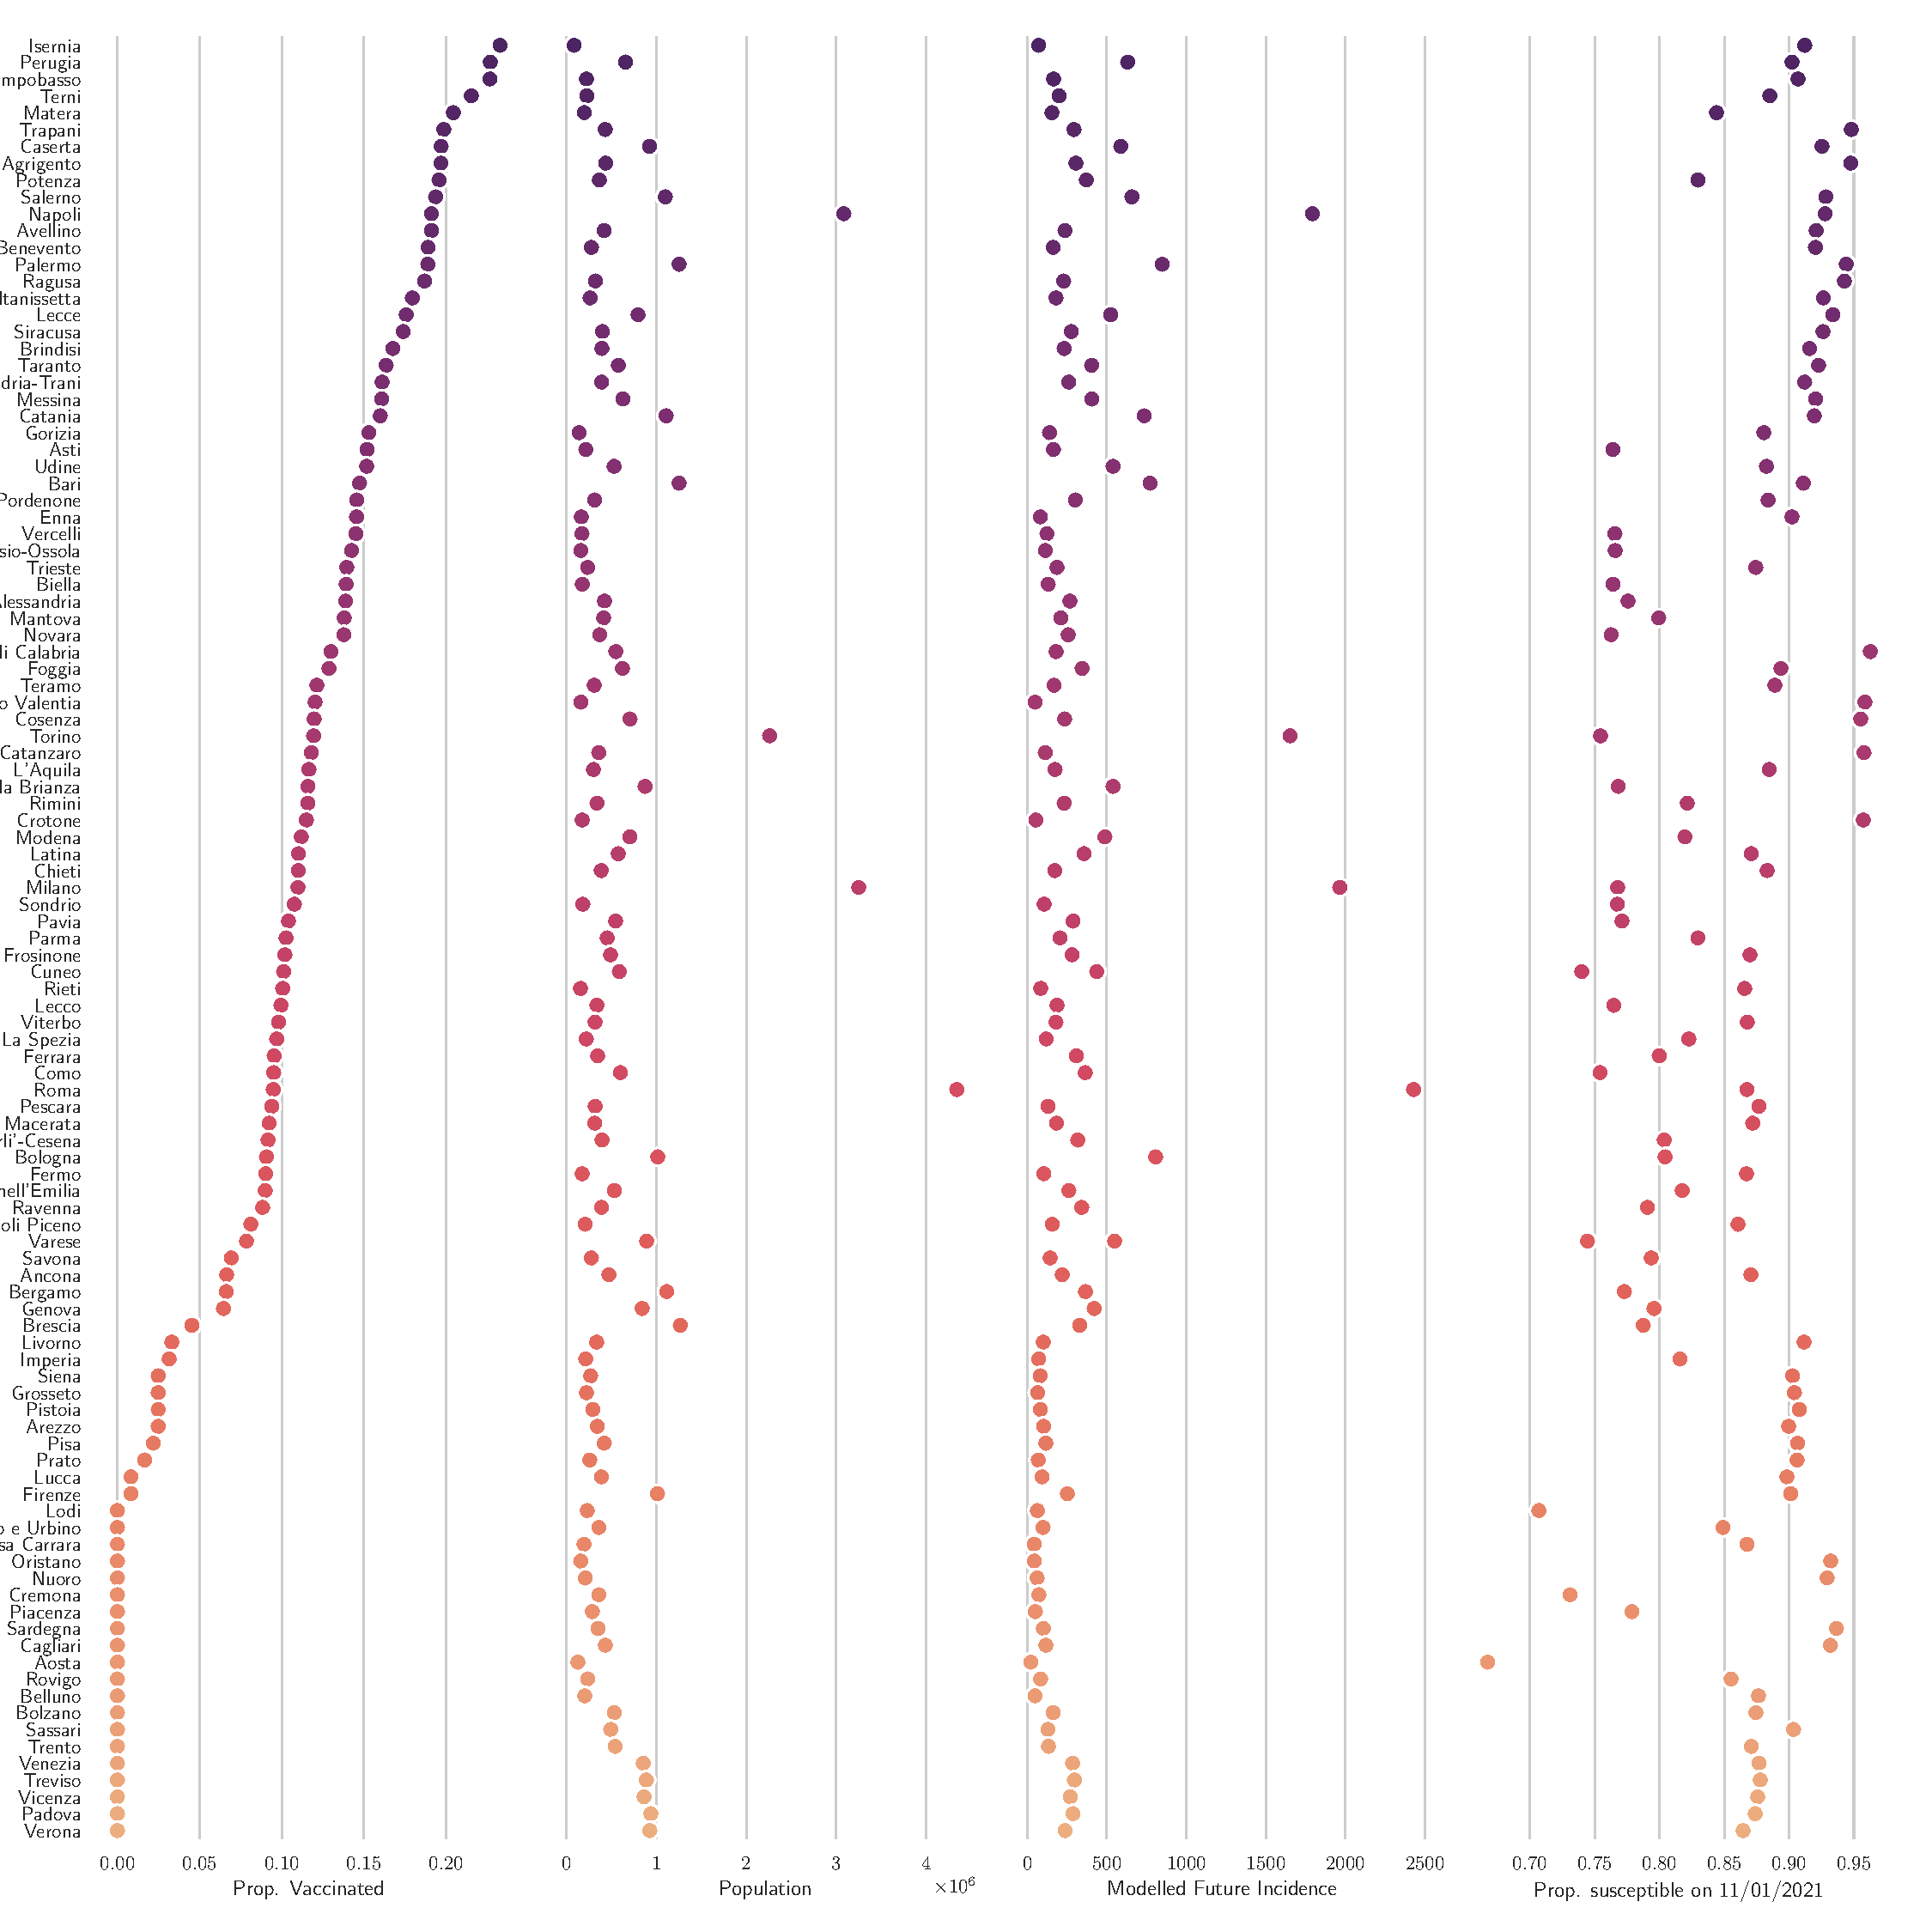
\includegraphics[width=\textwidth]{fig_italy-ocp/figuresSI/SI_scatter_Pessimistic.pdf}
    \caption[Control and co-variates for the pessimistic scenario]{Control and co-variates for the pessimistic scenario with a stockpile delivery of 479'700 vaccine doses.}
    \label{fig:OC_scatter_pessimistic}
\end{figure}

%\begin{figure}[!ht]
%    \centering
 %   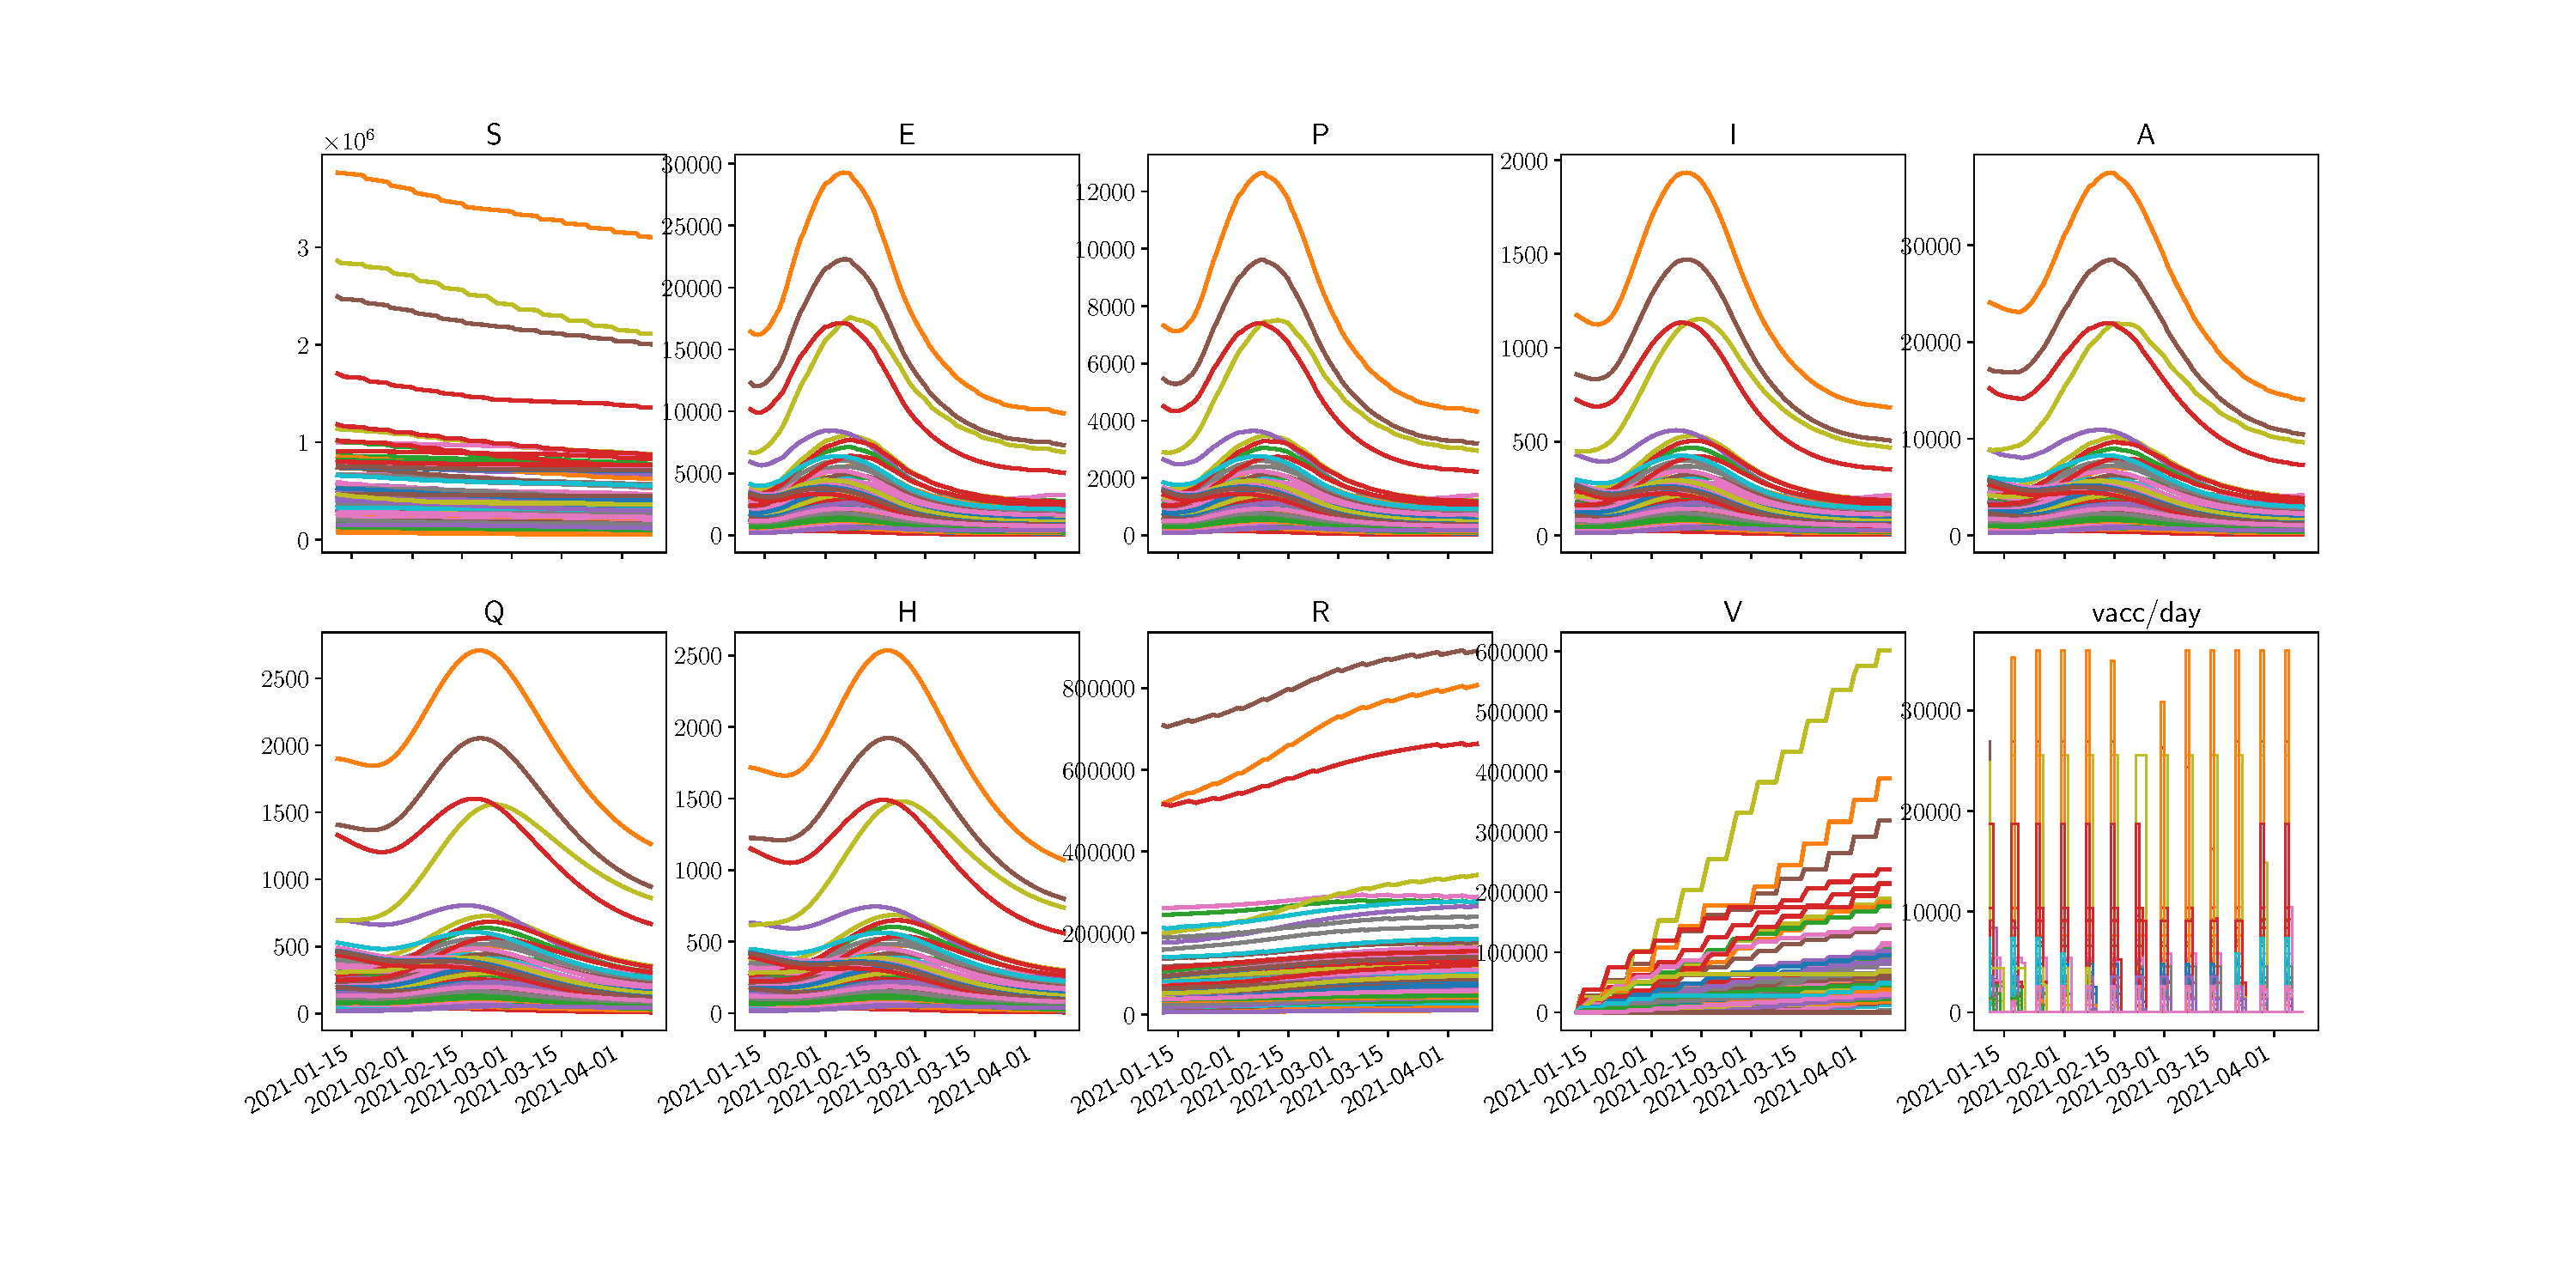
\includegraphics[width=\textwidth]{fig_italy-ocp/figuresSI/SI_all_states.pdf}
  %  \caption[Example of the dynamics in all compartments]{Example of the dynamics in all compartments for every node in the pessimistic scenario with a stockpile delivery of 479'700 doses. The lower right plot shows the control variable, the number of doses per day in each province.}
%    \label{fig:OC_ts_all}
%\end{figure}




